\documentclass{beamer}
\usepackage{lmodern}
\usepackage[utf8]{inputenc}


%\usepackage[latin1]{inputenc}
\usepackage[english]{babel}
\usepackage{amsmath}
\usepackage{cases}
\usepackage[makeroom]{cancel}
\usepackage{amsmath,tabu}
\usepackage[fleqn]{mathtools}
\usepackage[fleqn]{amsmath}
\usepackage{bm}
\usepackage{tikz}
\usepackage{enumitem}
\usepackage{wrapfig}
\usepackage{graphicx}
\usepackage{siunitx}
\usepackage{microtype}
\usepackage{array,tabularx}
\usepackage{float}
\usepackage{booktabs}
\usepackage{import}
\usepackage{cases}
\usepackage{graphicx,subfigure}
\usepackage{myUnitOfMeasure}
%\usepackage{myThermodynamics}
\usepackage{myMath}
\usepackage{mathtools}
\usepackage{gensymb}
\usepackage{xcolor}
\usepackage{url}
\usepackage{tabularx}
\usepackage{ltablex}
\usepackage{booktabs}
\usepackage{float}
\usepackage{listings}
\restylefloat{table} % with H force table position

\usepackage{enumerate}
\usepackage{multimedia}

% usefull for ltablex to split long tables in many pages
\keepXColumns

\DeclarePairedDelimiter\abs{\lvert}{\rvert}%

%\newcommand{\Fy}[1]{\text{F}_{y_{#1}}}

%\newcommand{\diameter}{\oslash}

%\newcommand{\todo}{\colorbox{cyan!60}{TODO}}

\renewcommand{\thesubsection}{\thesection.\arabic{subsection}}

\renewcommand{\arraystretch}{1.4}

\newcommand{\variable}[1]{\textcolor{blue}{#1}}

\newcommand{\paramtext}[1]{\textcolor{black!30!green}{#1}}

\newcommand{\terminal}[1]{\textcolor{black!30!cyan}{#1}}

\newcommand{\todo}{\colorbox{cyan!60}{TODO}}

\newcommand{\nut}{\nu_\text{T}}

\newcommand{\foam}[1]{{\ttfamily #1}}

\newcommand{\kepsilon}{$k\!-\!\varepsilon $ } 

\newcommand{\komegasst}{$k\!-\!\omega \, \text{SST} $ } 


\lstset{
	basicstyle=\fontsize{11}{13}\selectfont\ttfamily,
    frame=tb, % draw a frame at the top and bottom of the code block
    tabsize=4, % tab space width
    showstringspaces=false, % don't mark spaces in strings
    numbers=left, % display line numbers on the left
    commentstyle=\color{black!50!green}, % comment color
    keywordstyle=\color{blue!50!cyan}, % keyword color
    stringstyle=\color{black!30!red} % string color
}



\newcommand{\fakecaption}{%
  \vskip0.5\baselineskip
  \refstepcounter{table}%
  \tablename\ \thetable%
}


\usetheme{polimix}
 
\title[MRL TURBINE]{MRL TURBINE SIMULATION}
\subtitle{MODELLING TECHNIQUES FOR FLUID MACHINES}

\author[AR MB MB AC]{Andrea Rossi \and Marco Bonasegale \and Marco Belloli \and Alberto Casali}

\supervisor{Supervisor}{Gianluca Montenegro \quad Giacomo Persico}

\coadvisor{Co-Advisor}{Augusto Della Torre}
%\date[06/07/2018]{July 2018}
\date{}
\begin{document}

%%%%%%%%%%%%%%%%%%%%%%%%%%%%%%%%%%%%%%%%%%%%%%%%%%%%%%%%%%%%%%%%%%%%%%%%%%%%%%%%%%%%%%%%%%%%%%%%%%%%%%%%%%%%%%%%%%%%

\begin{frame}
\titlepage
\end{frame}

\addtocounter{framenumber}{-1}

%%%%%%%%%%%%%%%%%%%%%%%%%%%%%%%%%%%%%%%%%%%%%%%%%%%%%%%%%%%%%%%%%%%%%%%%%%%%%%%%%%%%%%%%%%%%%%%%%%%%%%%%%%%%%%%%%%%%

%\begin{frame}
%\frametitle{Sommario}
%\tableofcontents
%\end{frame}
%







%%%%%%%%%%%%%%%%%%%%%%%%%%%%%%%%%%%%%%%%%%%%%%%%%%%%%%%%%%%%%%%%%%%%%%%%%%%%%%%%%%%%%%%%%%%%%%%%%%%%%%%%%%%%%%%%%%%
\section{Introduction}

\begin{frame}
\frametitle{Introduction}
The MRL (Momentum Reversal and Lift) Turbine is a hydraulic machine.
Problem data are:
\begin{itemize}
\item[$\cdot$] Inlet flow velocity of $1\ms$;
\item[$\cdot$] shaft rotational speed of $100 \, \text{rpm}$;
\item[$\cdot$] blades counter rotational speed of $50 \, \text{rpm}$;
\item[$\cdot$] geometry of the problem.
\end{itemize}

\begin{center}
\begin{figure}
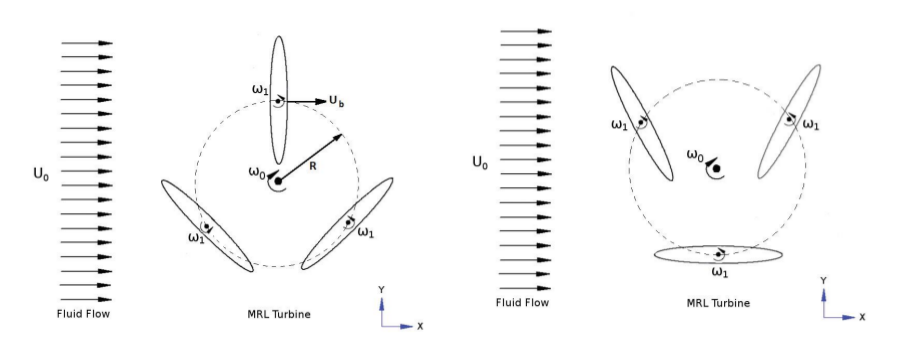
\includegraphics[width=0.9\textwidth]{images/flow.png} 

\end{figure}
\end{center}


\end{frame}

%%%%%%%%%%%%%%%%%%%%%%%%%%%%%%%%%%%%%%%%%%%%%%%%%%%%%%%%%%%%%%%%%%%%%%%%%%%%%%%%%%%%%%%%%%%%%%%%%%%%%%%%%%%%%%%%%%%
\section{In class work}

%%%%%%%%%%%%%%%%%%%%%%%%%%%%%%%%%%%%%%%%%%%%%%
\begin{frame}
\frametitle{In class work - mesh generation}
The steps for the mesh generation are:
\begin{itemize}
\item[$\cdot$] \foam{surfaceTransformPoints} to scale of the STL files;
\item[$\cdot$] \foam{blockMesh} and \foam{snappyHexMesh} of each regions and blades;
\item[$\cdot$] \foam{mergeMesh} to marge the 5 previous regions;
\item[$\cdot$] \foam{extrudeMesh} to reconstruct a 2D mesh;
\item[$\cdot$] \foam{refineWallLayer} to reduce layers size near the blades.
\end{itemize}

\begin{figure}[H]
\centering
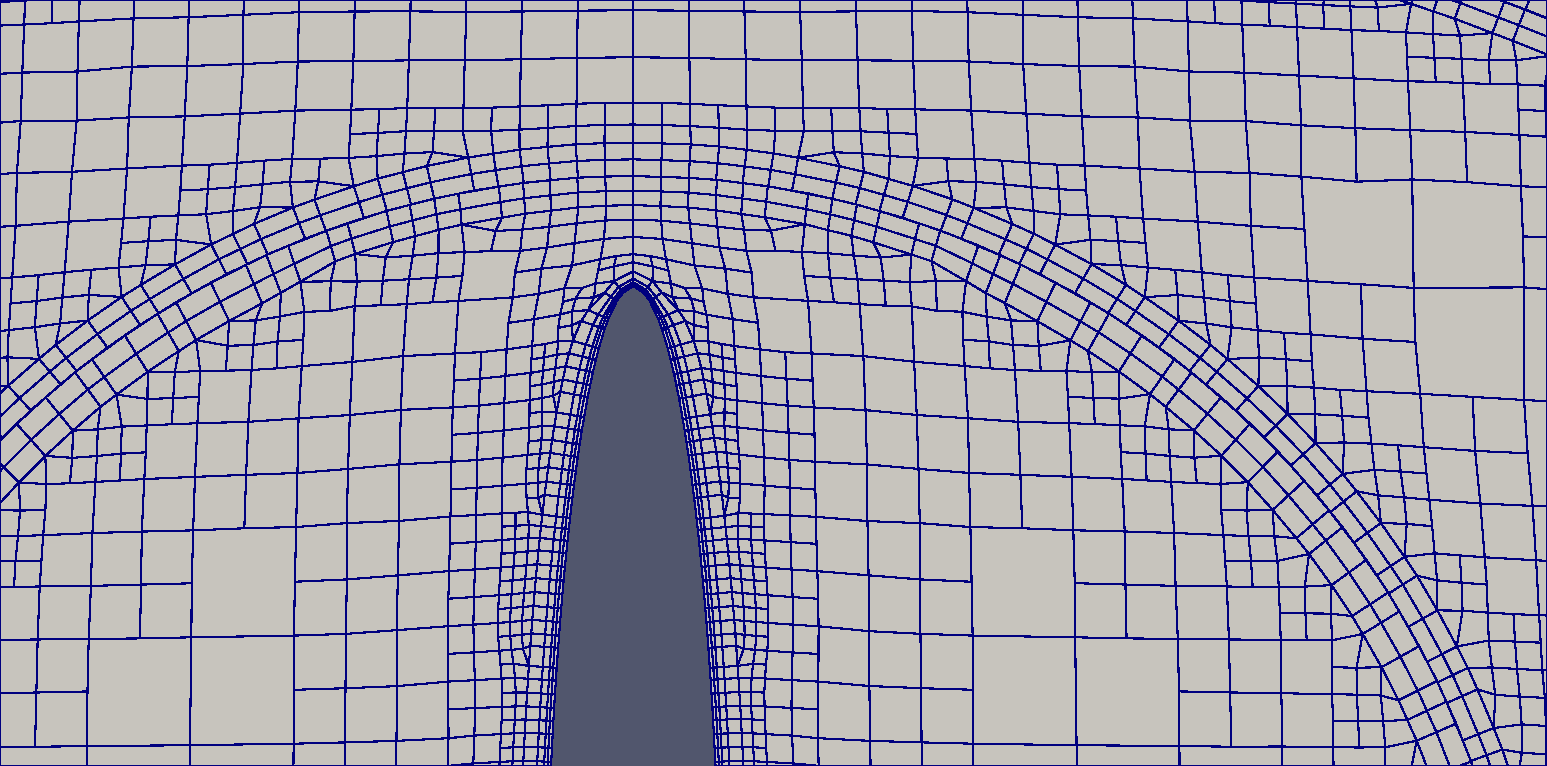
\includegraphics[height=4cm]{images/inclass/mesh40.pdf}
\end{figure}

\end{frame}

%%%%%%%%%%%%%%%%%%%%%%%%%%%%%%%%%%%%%%%%%%%%%%
\begin{frame}
\frametitle{In class work - the boundaries}

\textbf{Inlet} \quad velocity is fixed to $1\ms$ while all the other quatities are calculated according to the physics of the simulation.
\\
\textbf{Outlet} \quad relative pressure is fixed to $0 \,\text{m}^2/\text{s}^2$ (atmosferic pressure) while all the others are free to change according to upstream evolution.
\\
\textbf{Upper surface} \quad relative pressure is fixed to $0 \,\text{m}^2/\text{s}^2$ (atmosferic pressure) while all the others are free to change according to the flow evolution.
\\
\textbf{Bottom wall} \quad velocity is set to no slip condition to mimic adherence and so boundary layer evolution. Pressure is set to \foam{zeroGradient}, typical condition in B.L. All the others are free.
\\\textbf{Blades} \quad a similar no slip condition for moving walls is applied for the velocity. B.L. is isobaric without gradient of pressure. All the others depends on flow solution.

\end{frame}


%%%%%%%%%%%%%%%%%%%%%%%%%%%%%%%%%%%%%%%%%%%%%%
\begin{frame}
\frametitle{In class work - the simulation results}

\begin{figure}[H]
\subfigure[Pressure at 2.4]{\includegraphics[width=5cm]{images/inclass/{pfield2.4sec}.png}}
\hfill
\subfigure[Velocity at 2.4]{\includegraphics[width=5cm]{images/inclass/{velocityfield2.4sec}.png}}
\end{figure}

\begin{table}[H]
\centering
\begin{tabular}{lr}
\toprule
Power (Pressure) [W]     & $\round{4.84602561871}$   \\ \midrule
Power (Shear stress) (W) & $\round{-0.253811271949}$ \\
Power (Total) [W]        & $\round{4.59221434676}$   \\ \bottomrule
\end{tabular}
\caption{Mean power between 1.8 and 2.4}
\label{table:inclass-power}
\end{table}

\end{frame}

%%%%%%%%%%%%%%%%%%%%%%%%%%%%%%%%%%%%%%%%%%%%%%
%%%%%%%%%%%%%%%%%%%%%%%%%%%%%%%%%%%%%%%%%%%%%%
\section{Mesh sensitivity analysis}

%%%%%%%%%%%%%%%%%%%%%%%%%%%%%%%%%%%%%%%%%%%%%%
\begin{frame}
\frametitle{Mesh sensitivity analysis}

We have performed the sensibility analysis with two different kind of grid:
\begin{itemize}
\item[$\cdot$] mesh without refinement region around blades;
\item[$\cdot$] mesh with refinement regiorn around blades.
\end{itemize}

\begin{figure}
\subfigure[Mesh without refinement region]{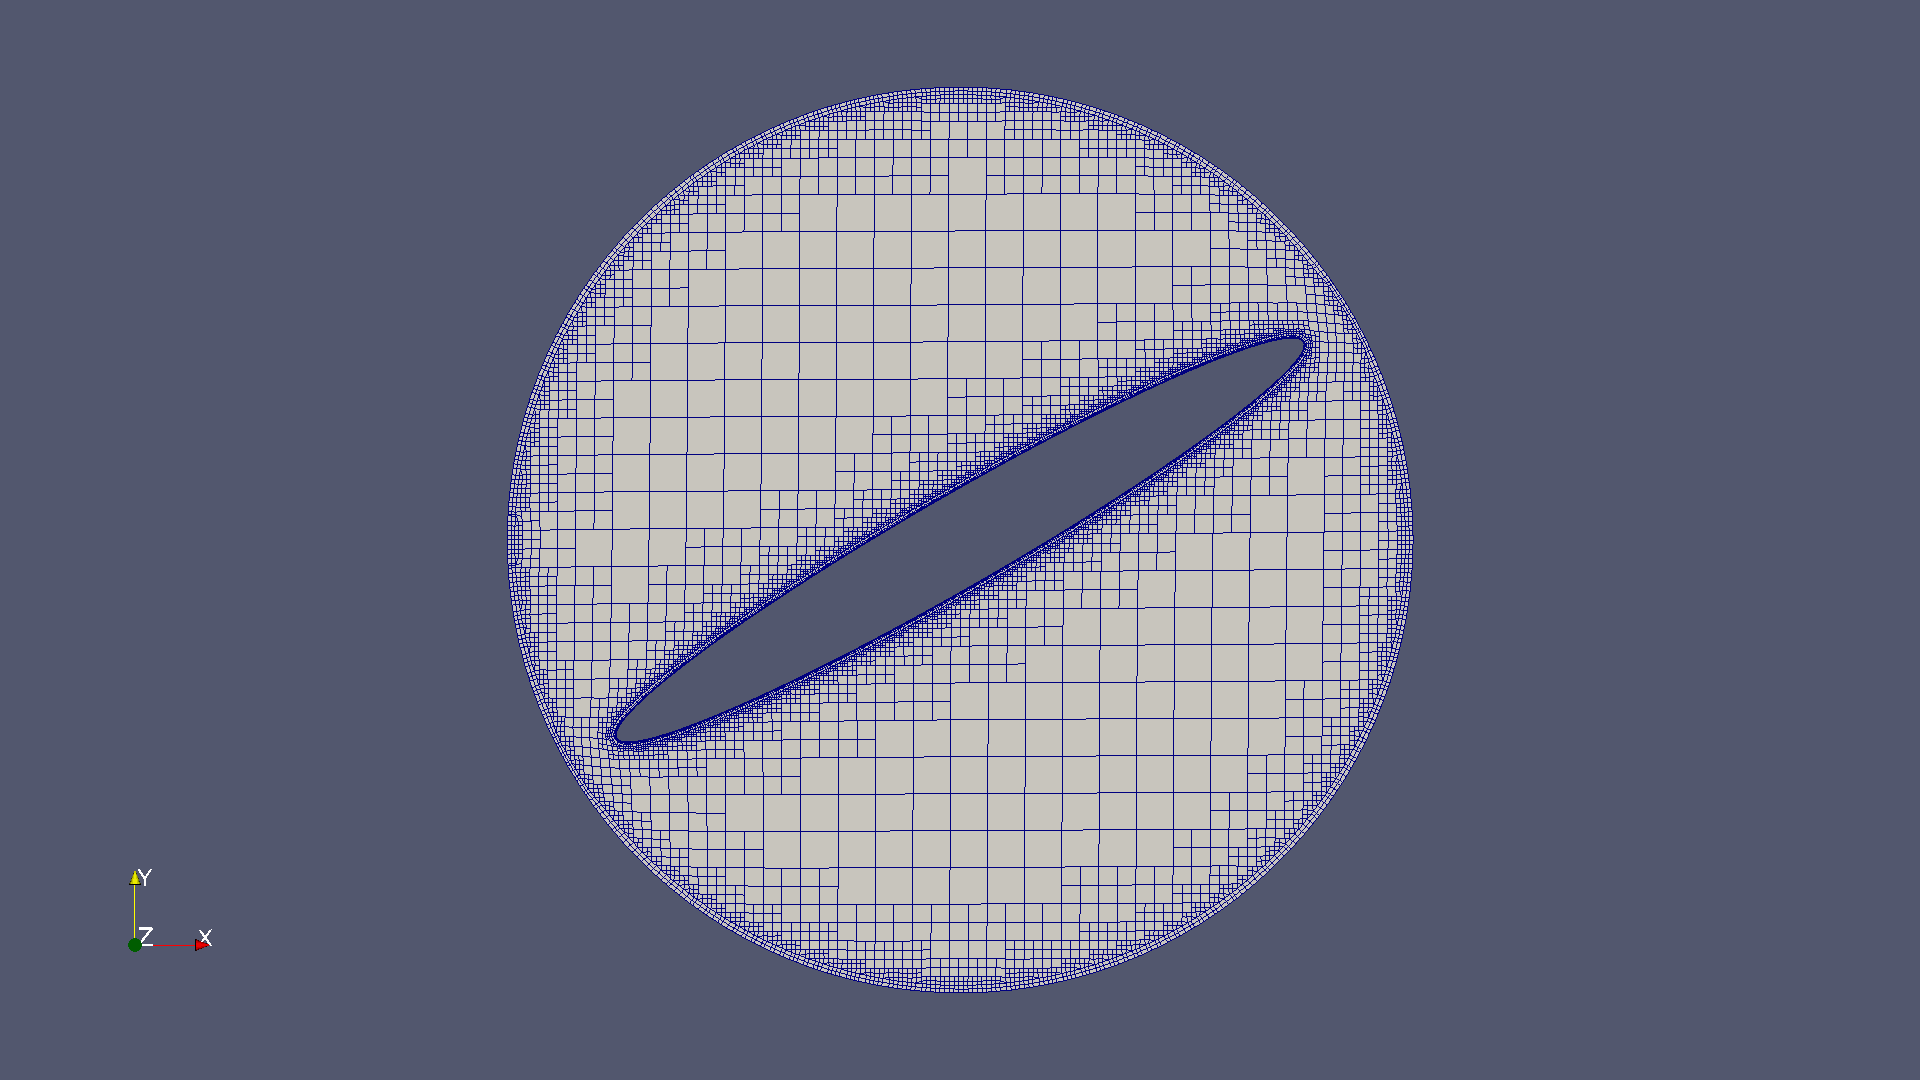
\includegraphics[width=5cm]{images/meshsensitivity/mesh120-blade0-noregion.png}}
\hfill
\subfigure[Mesh with refinement region]{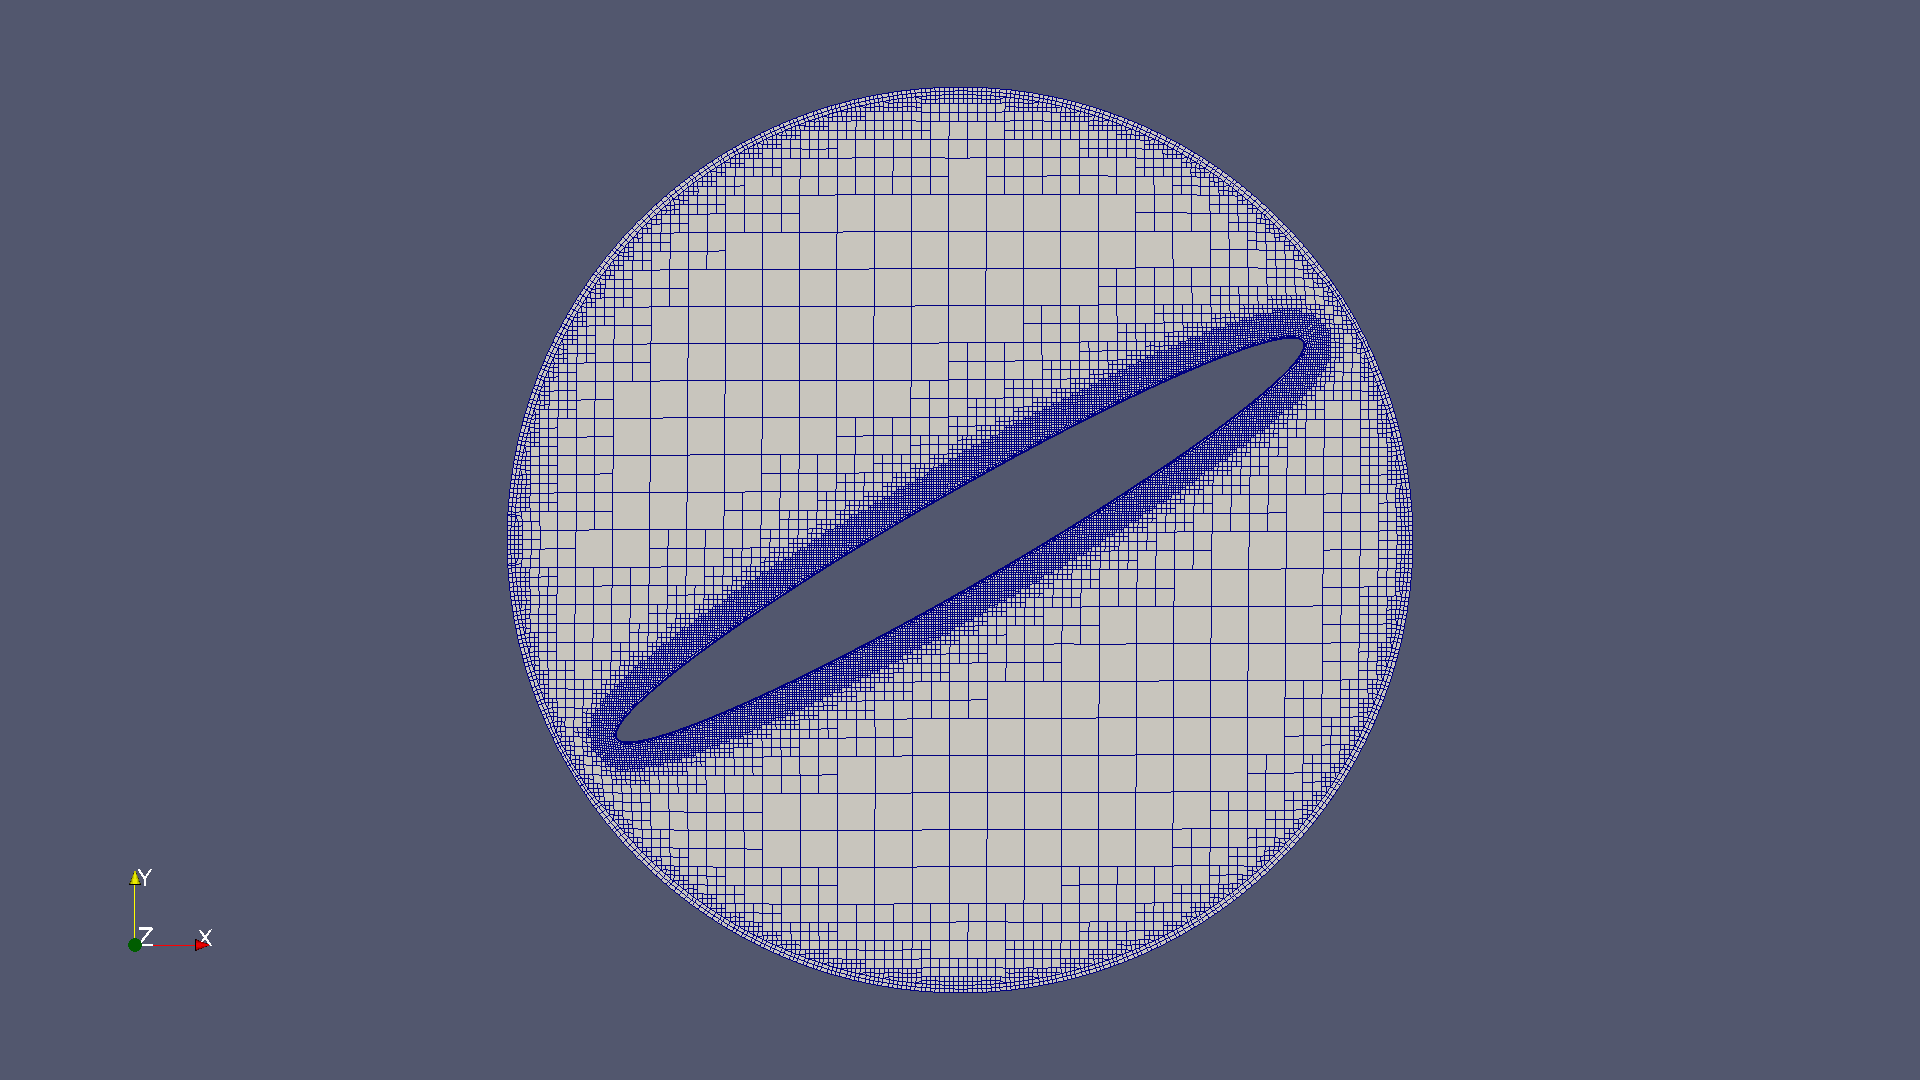
\includegraphics[width=5cm]{images/meshsensitivity/mesh120-blade0-region.png}}
\end{figure}

\end{frame}


%%%%%%%%%%%%%%%%%%%%%%%%%%%%%%%%%%%%%%%%%%%%%%
\begin{frame}
\frametitle{Mesh sensitivity analysis}

We have improved the number of cells acting on the refinement of the y axis.
We have started from 20 cells and have arrived to 160 cells.

\begin{table}[H]
\centering
%\begin{tabular}{@{}lrr@{}}
\begin{tabular}{lrr}
\toprule
         & Without region & With region \\ \midrule
Mesh 20  & 10328          & 10328      \\
Mesh 40  & 24066          & 25275      \\
Mesh 60  & 40462          & 44380      \\
Mesh 80  & 58877          & 66785      \\
Mesh 120 & 103384         & 124366      \\
Mesh 160 & 156791         & 196676      \\ \bottomrule
\end{tabular}
\end{table}

\end{frame}



%%%%%%%%%%%%%%%%%%%%%%%%%%%%%%%%%%%%%%%%%%%%%%
\begin{frame}
\frametitle{Mesh sensitivity analysis}

To perform the analysis we have considered:
\begin{itemize}
\item[$\cdot$] total power;
\item[$\cdot$] total power components ($p, \tau$);
\item[$\cdot$] total pressure drop (work and losses).
\end{itemize}


\begin{figure}[H]
\centering
\subfigure[Without refinement]{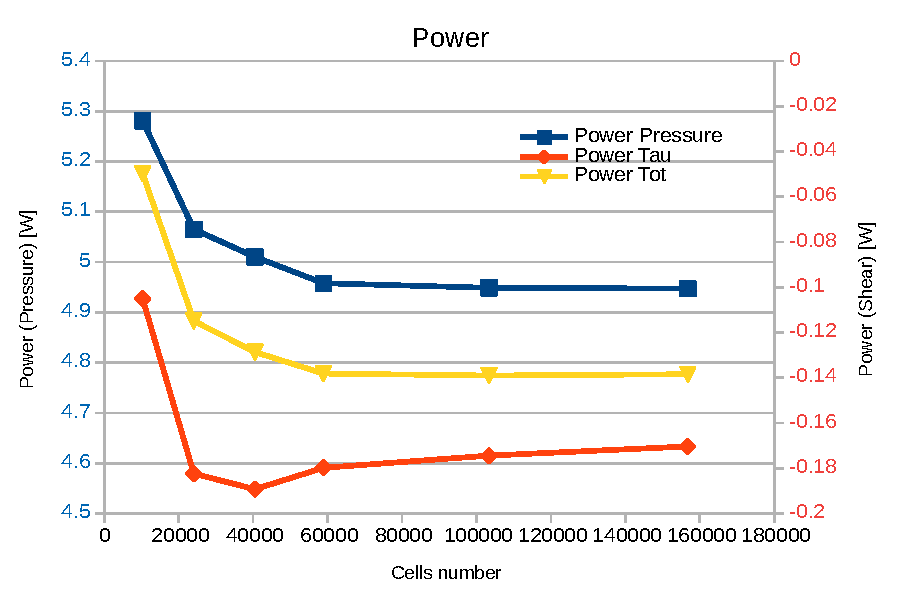
\includegraphics[width=5cm]{{images/meshsensitivity/mesh_sensitivity_andre}.pdf}}
\subfigure[With refinement]{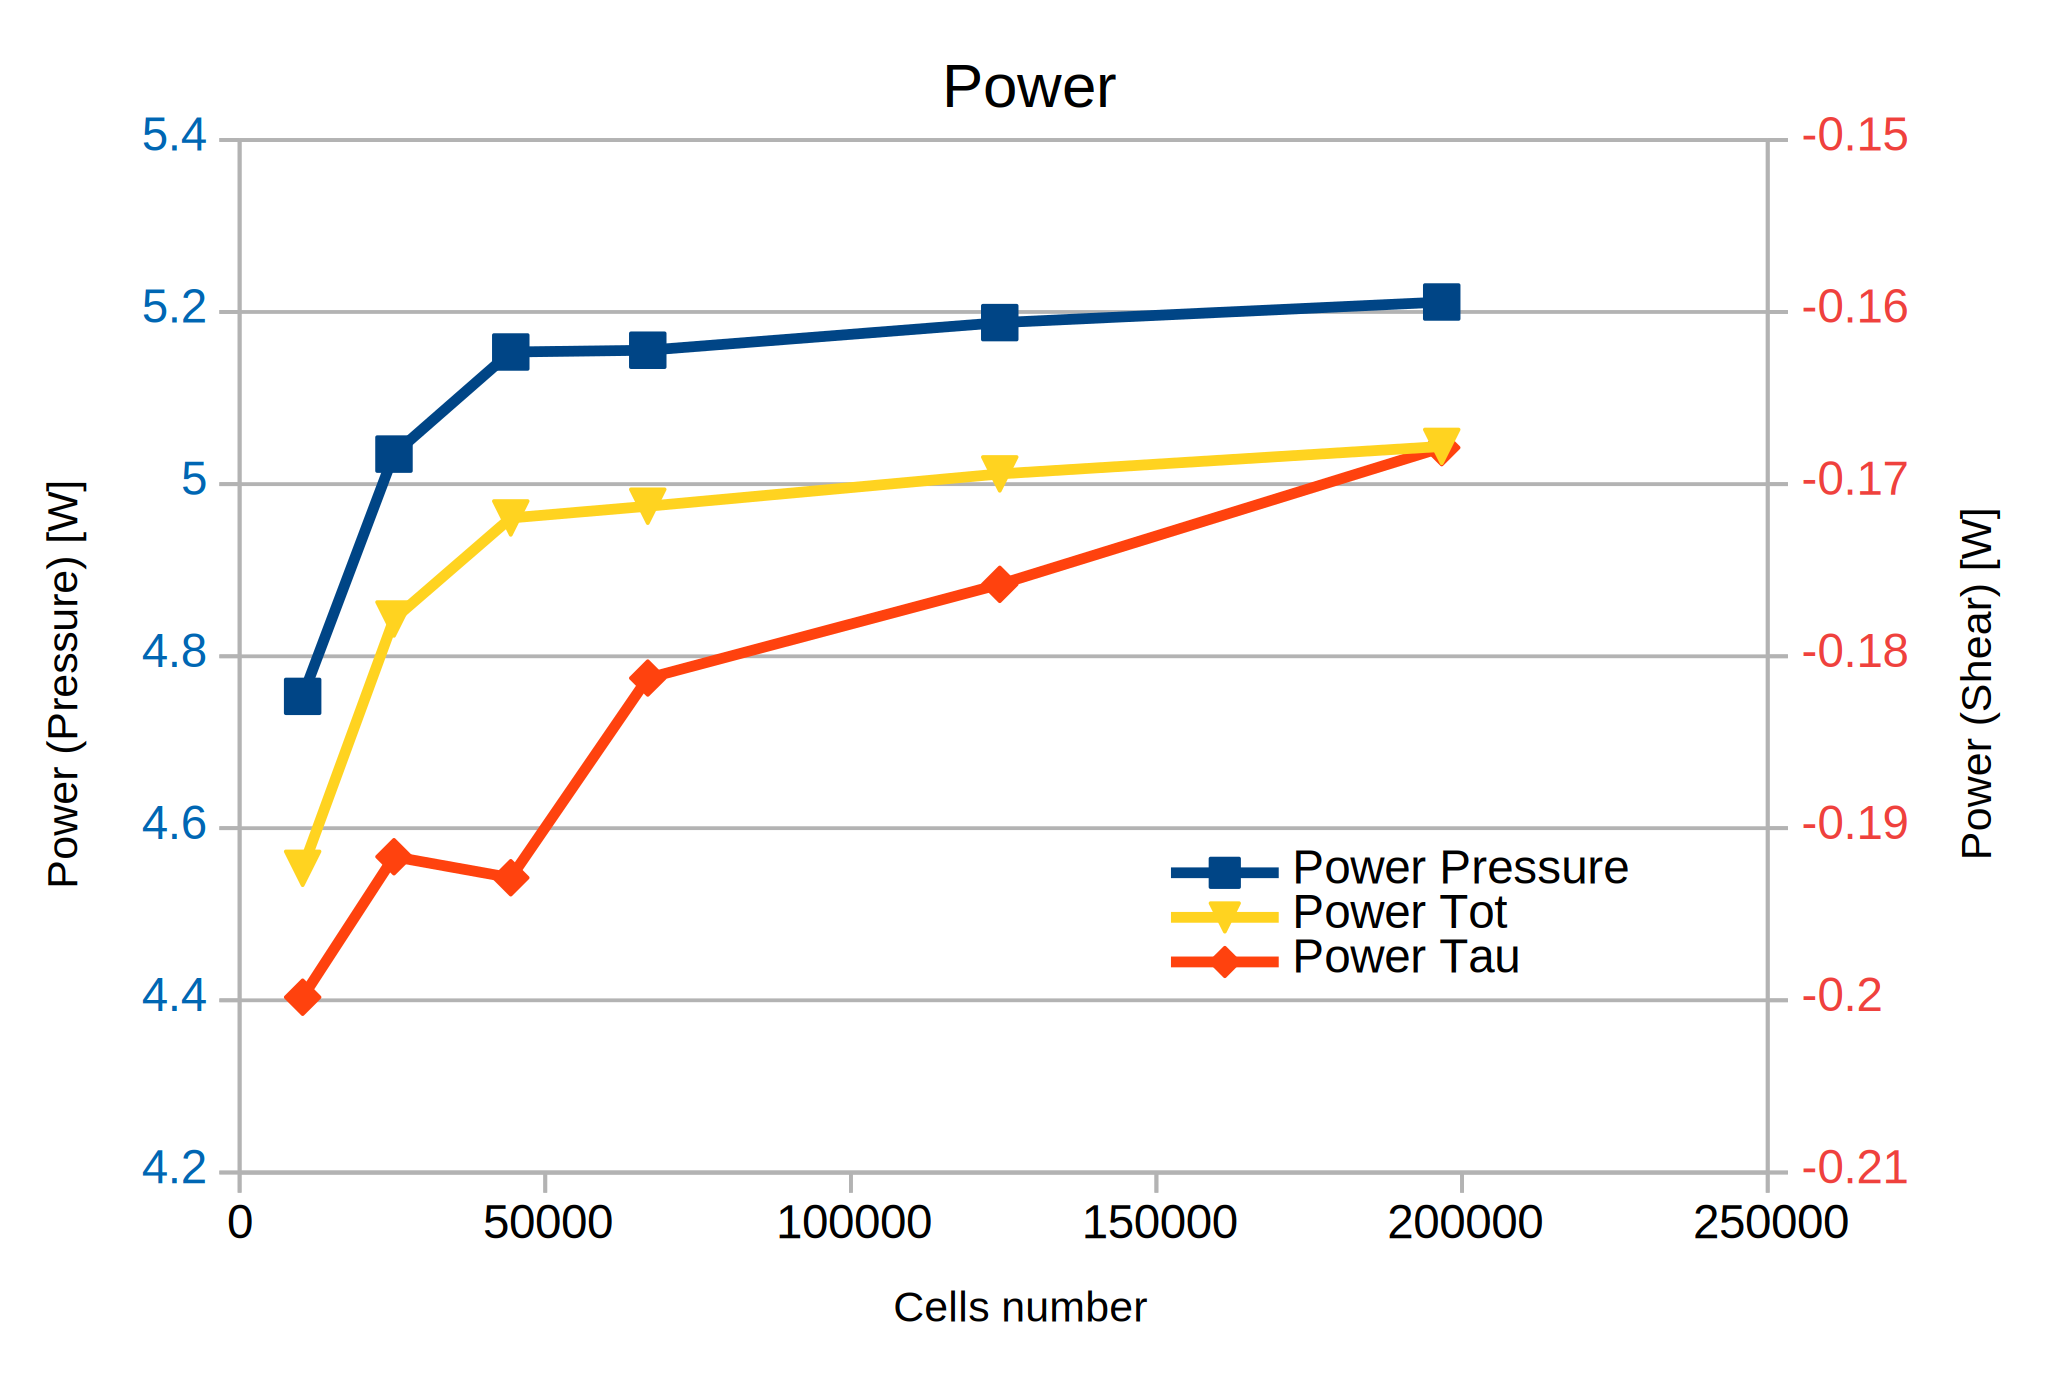
\includegraphics[width=5cm]{{images/meshsensitivity/mesh_sensitivity_marco}.pdf}}
%\caption{Total pressure drop between inlet and outlet at 2.4 seconds.}
%\label{fig:meshsensityvity-totalpressure-case2}
\end{figure}

%\begin{figure}[H]
%\centering
%\subfigure[Without refinement]{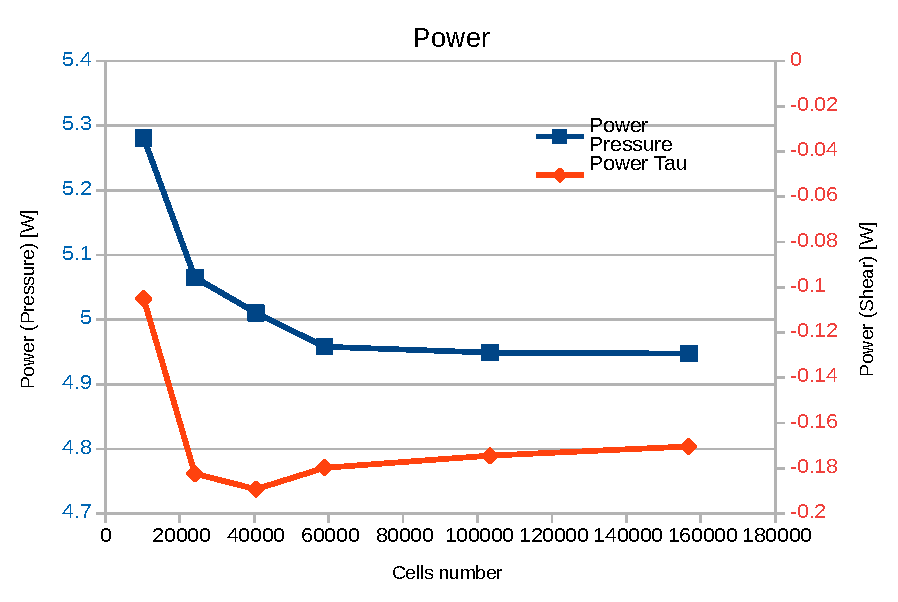
\includegraphics[width=5cm]{images/meshsensitivity/power-ptau-noregion}}
%\subfigure[With refinement]{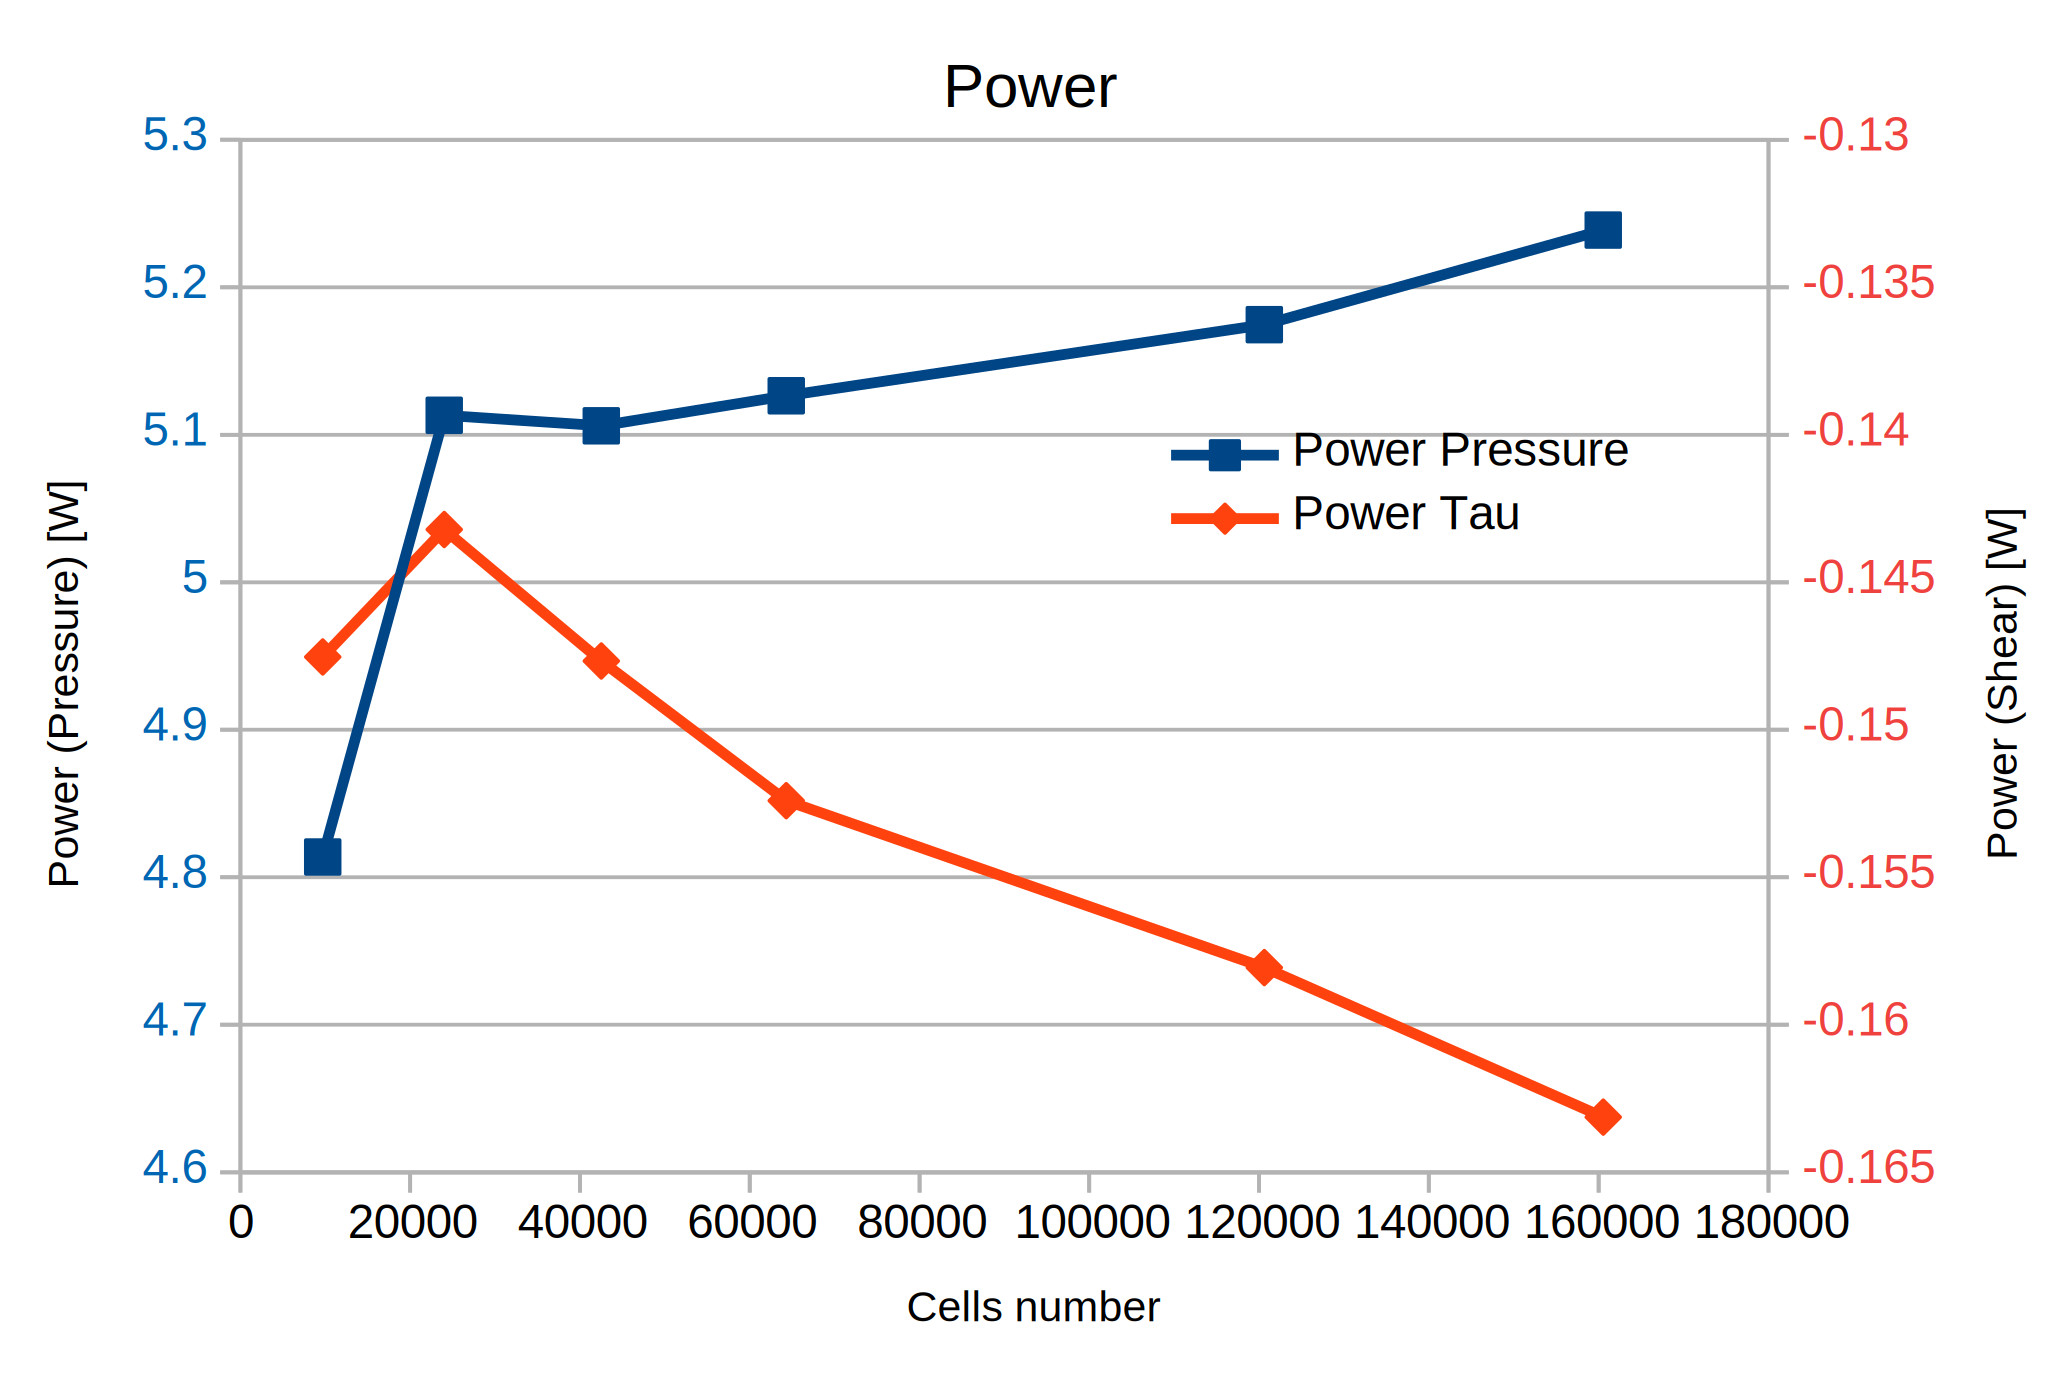
\includegraphics[width=5cm]{images/meshsensitivity/power-ptau-region}}
%%\caption{Average power in time between 1.8 and 2.4 seconds}
%%\label{fig:meshsensityvity-power-ptau}
%\end{figure}

\end{frame}


%%%%%%%%%%%%%%%%%%%%%%%%%%%%%%%%%%%%%%%%%%%%%%
\begin{frame}
\frametitle{Mesh sensitivity analysis}

For the total pressure drop we have considered the difference between the average at inlet and outlet at time $2.4 \s$


\begin{figure}[htbp]
\centering
\subfigure[Without refinement]{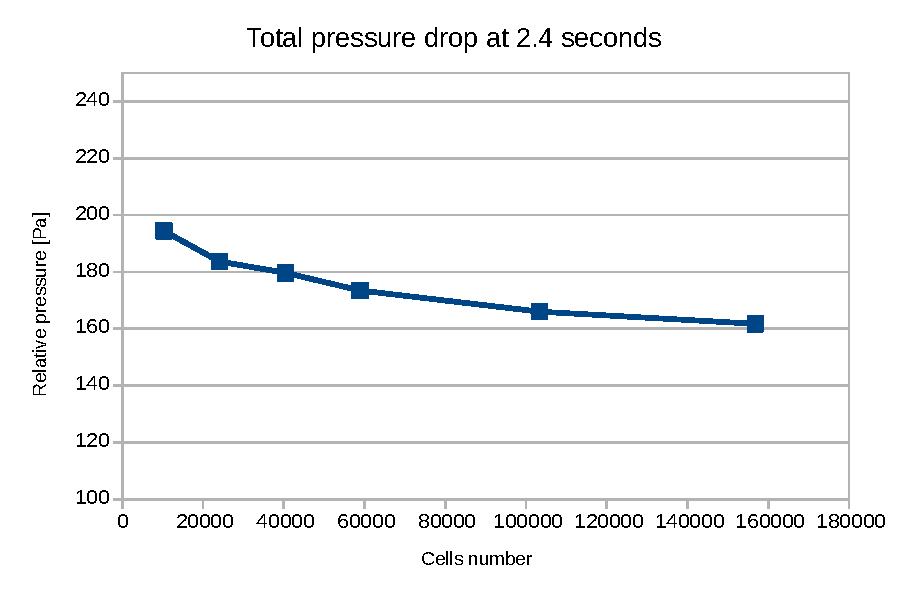
\includegraphics[width=5cm]{{images/meshsensitivity/totalpdrop-2.4-noregion}.pdf}}
\subfigure[With refinement]{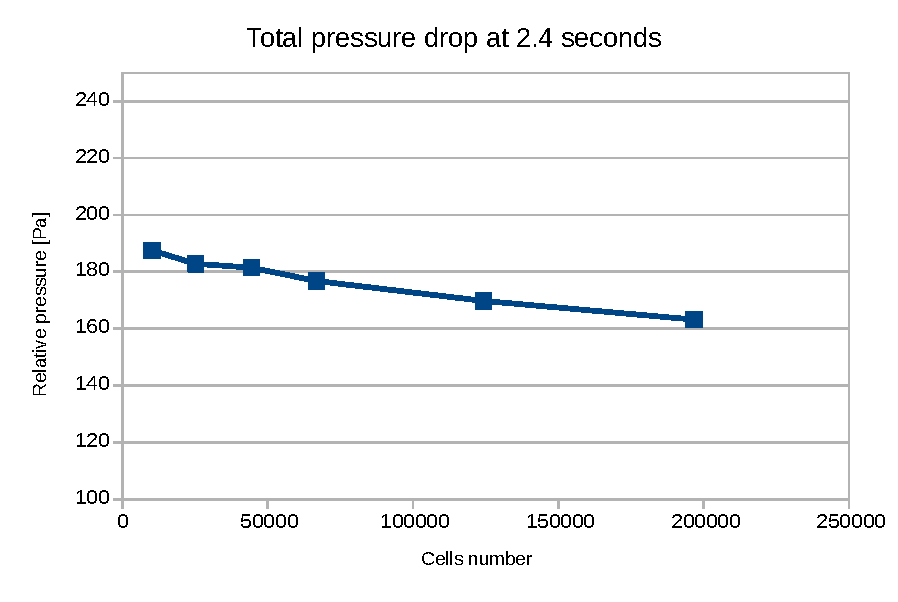
\includegraphics[width=5cm]{{images/meshsensitivity/totalpdrop-2.4-region}.pdf}}
%\caption{Total pressure drop between inlet and outlet at 2.4 seconds.}
%\label{fig:meshsensityvity-totalpressure-case2}
\end{figure}

\end{frame}




%%%%%%%%%%%%%%%%%%%%%%%%%%%%%%%%%%%%%%%%%%%%%%
\begin{frame}
\frametitle{Mesh sensitivity analysis - final mesh}

The result of the sensitivity analysis suggested up to adopt mesh 120 which is tradeoff betweeen:
\begin{itemize}
\item[$\cdot$] computational cost;
\item[$\cdot$] results reliability.
\end{itemize}

\begin{figure}[hbtp]
\centering
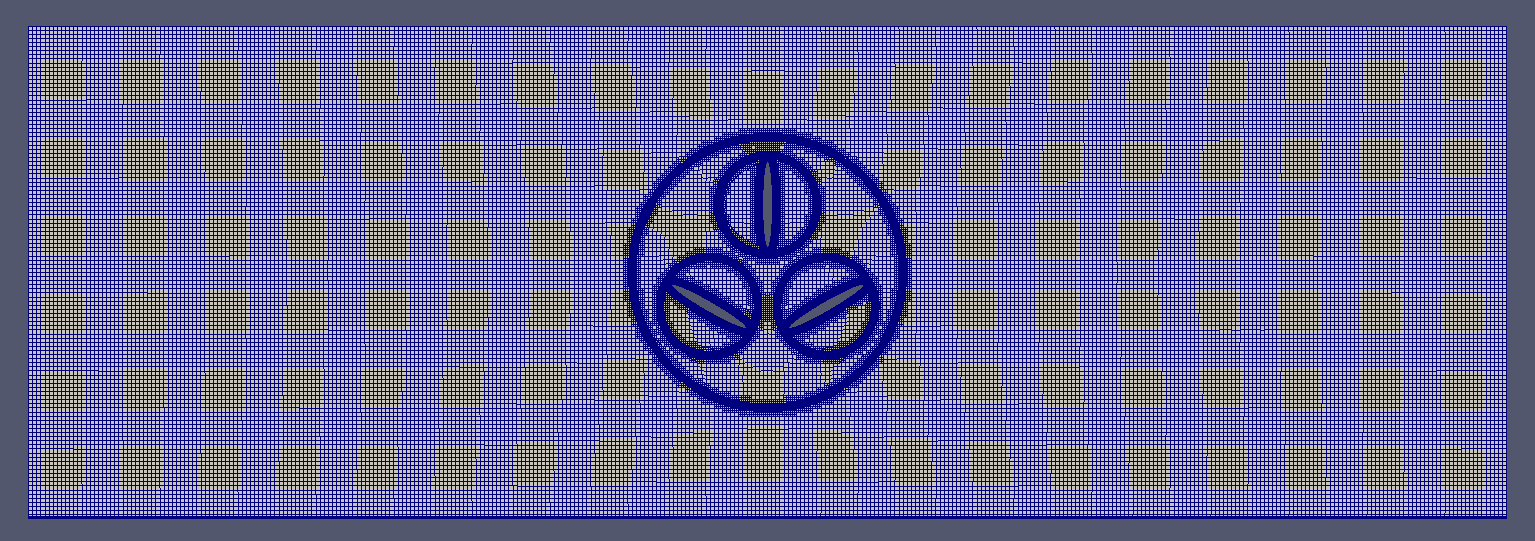
\includegraphics[width=11cm]{images/mesh-120/view-full.png}
%\caption{Full view of the mesh}
\end{figure}

\end{frame}


%%%%%%%%%%%%%%%%%%%%%%%%%%%%%%%%%%%%%%%%%%%%%%
\begin{frame}
\frametitle{Mesh sensitivity analysis - final mesh}

\begin{figure}[htbp]
\centering
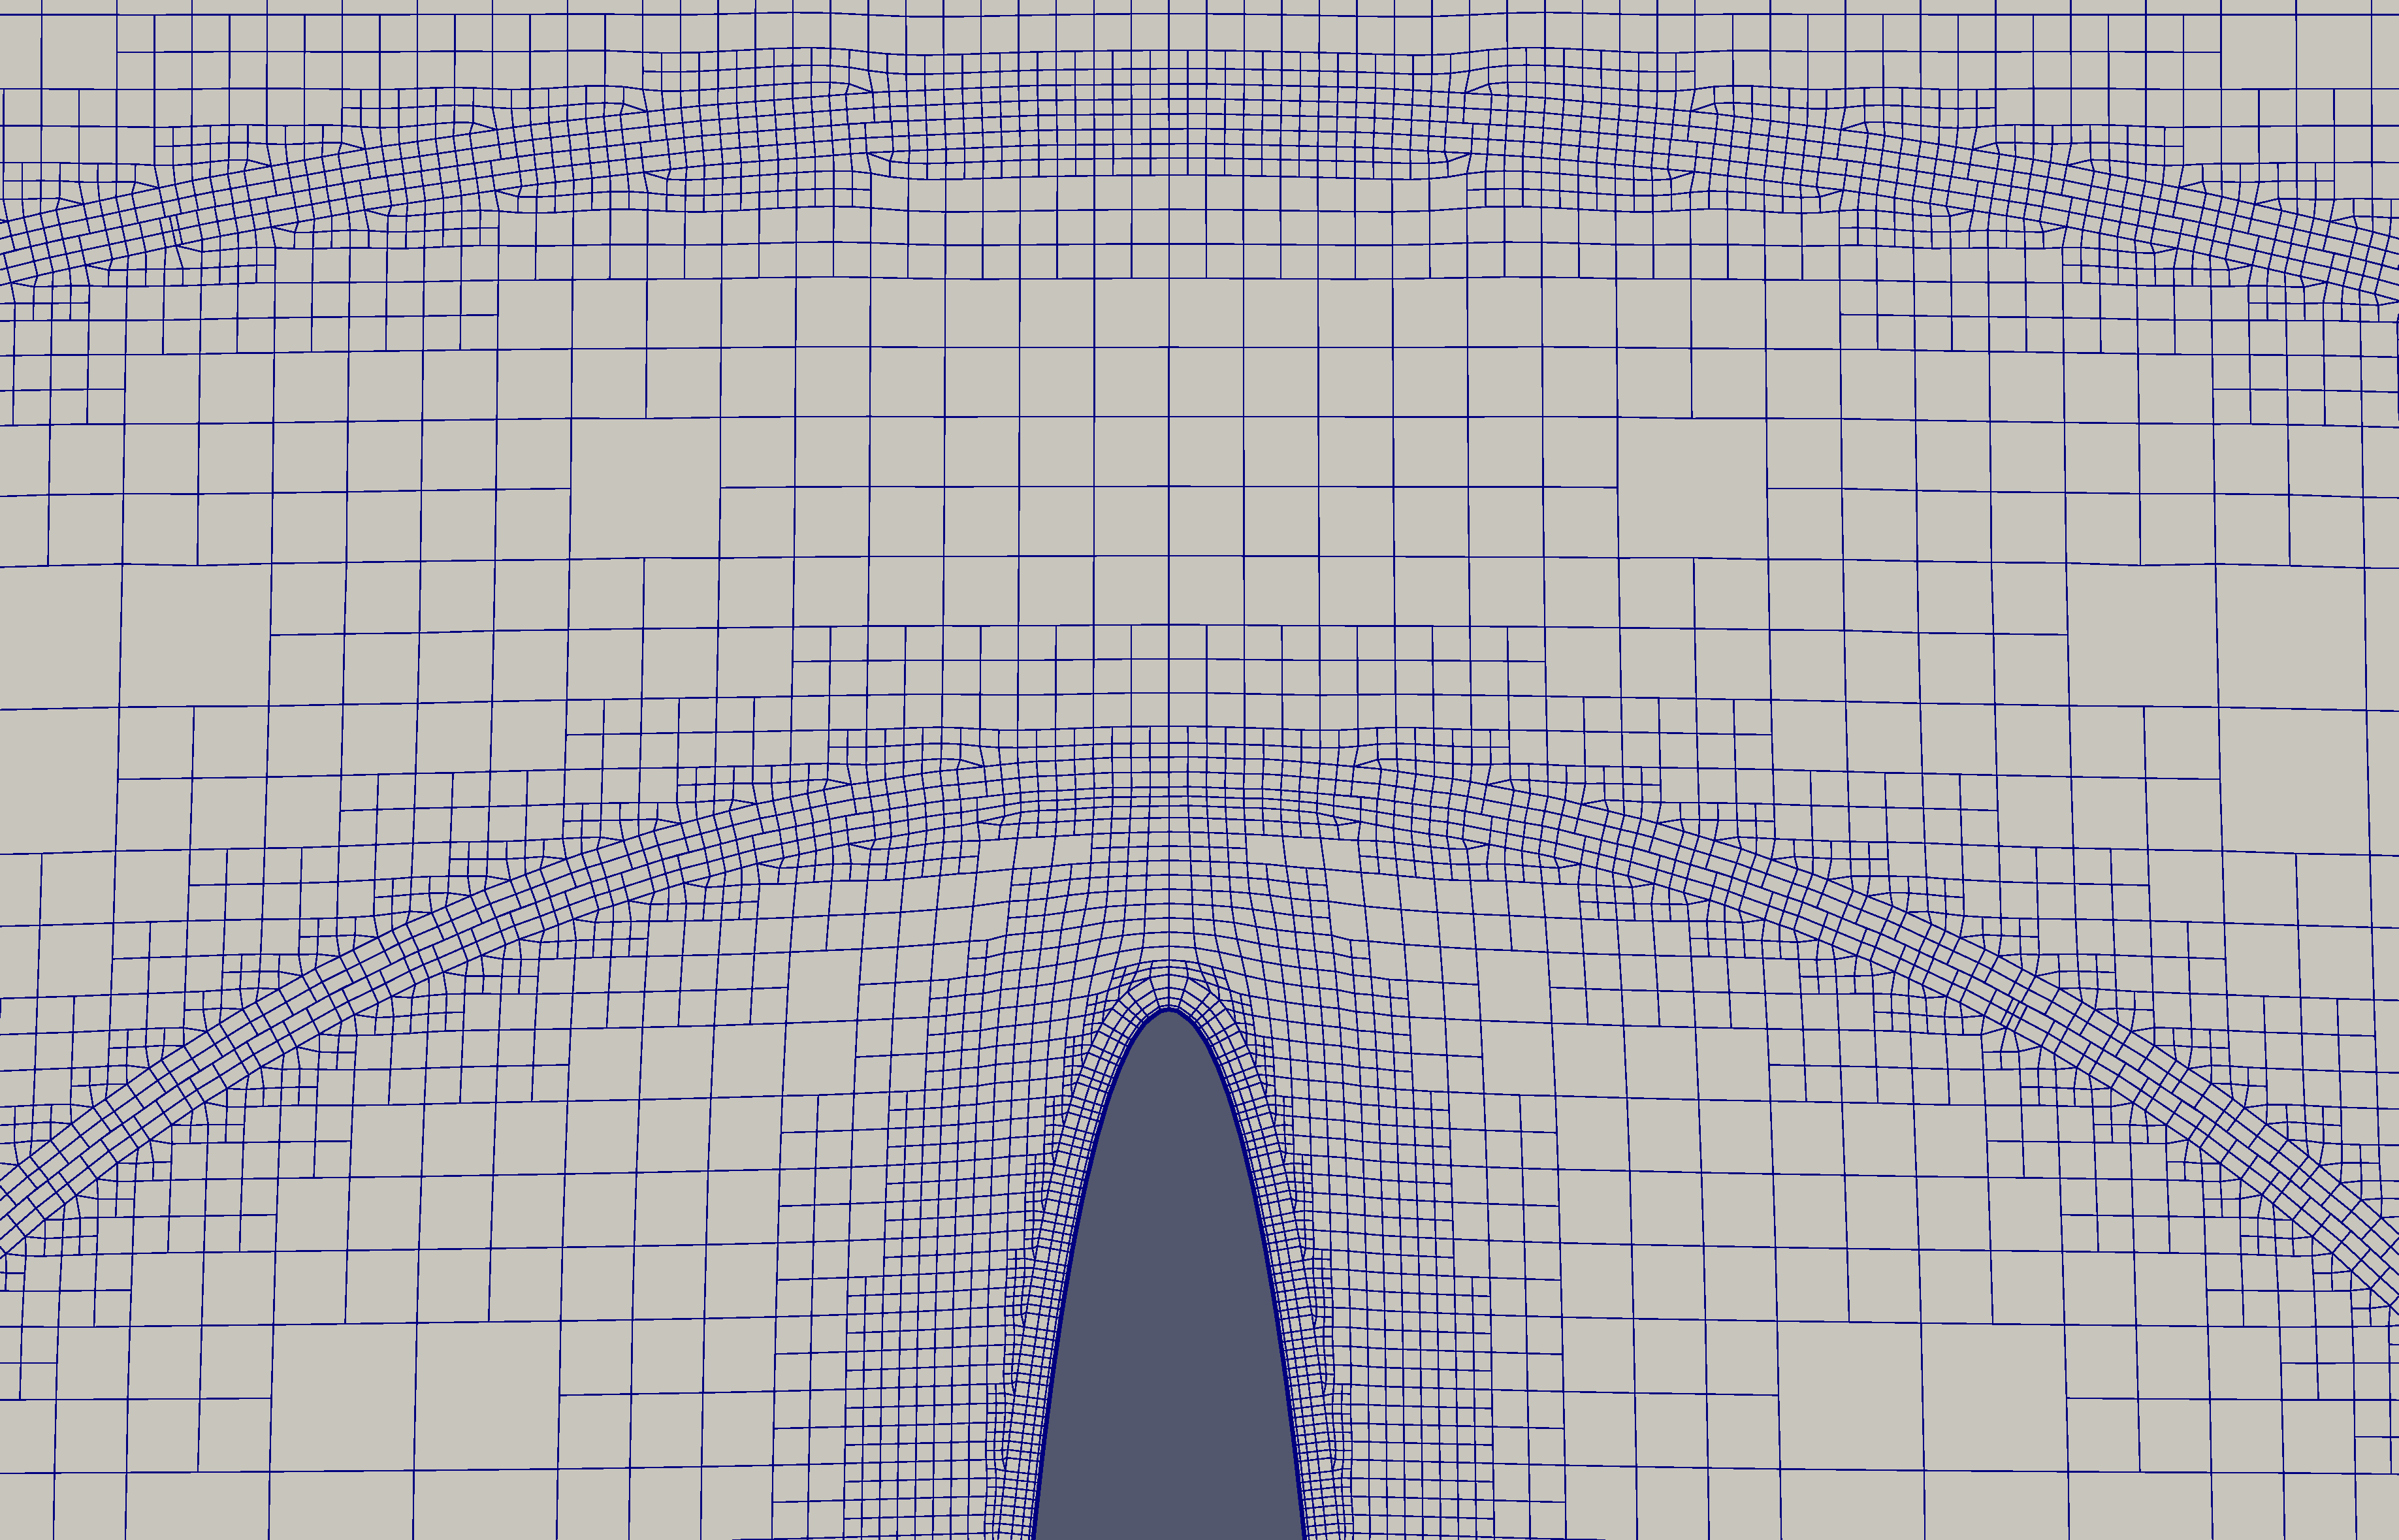
\includegraphics[width=5cm]{{images/mesh-120/view-bladetip}.pdf}
\quad
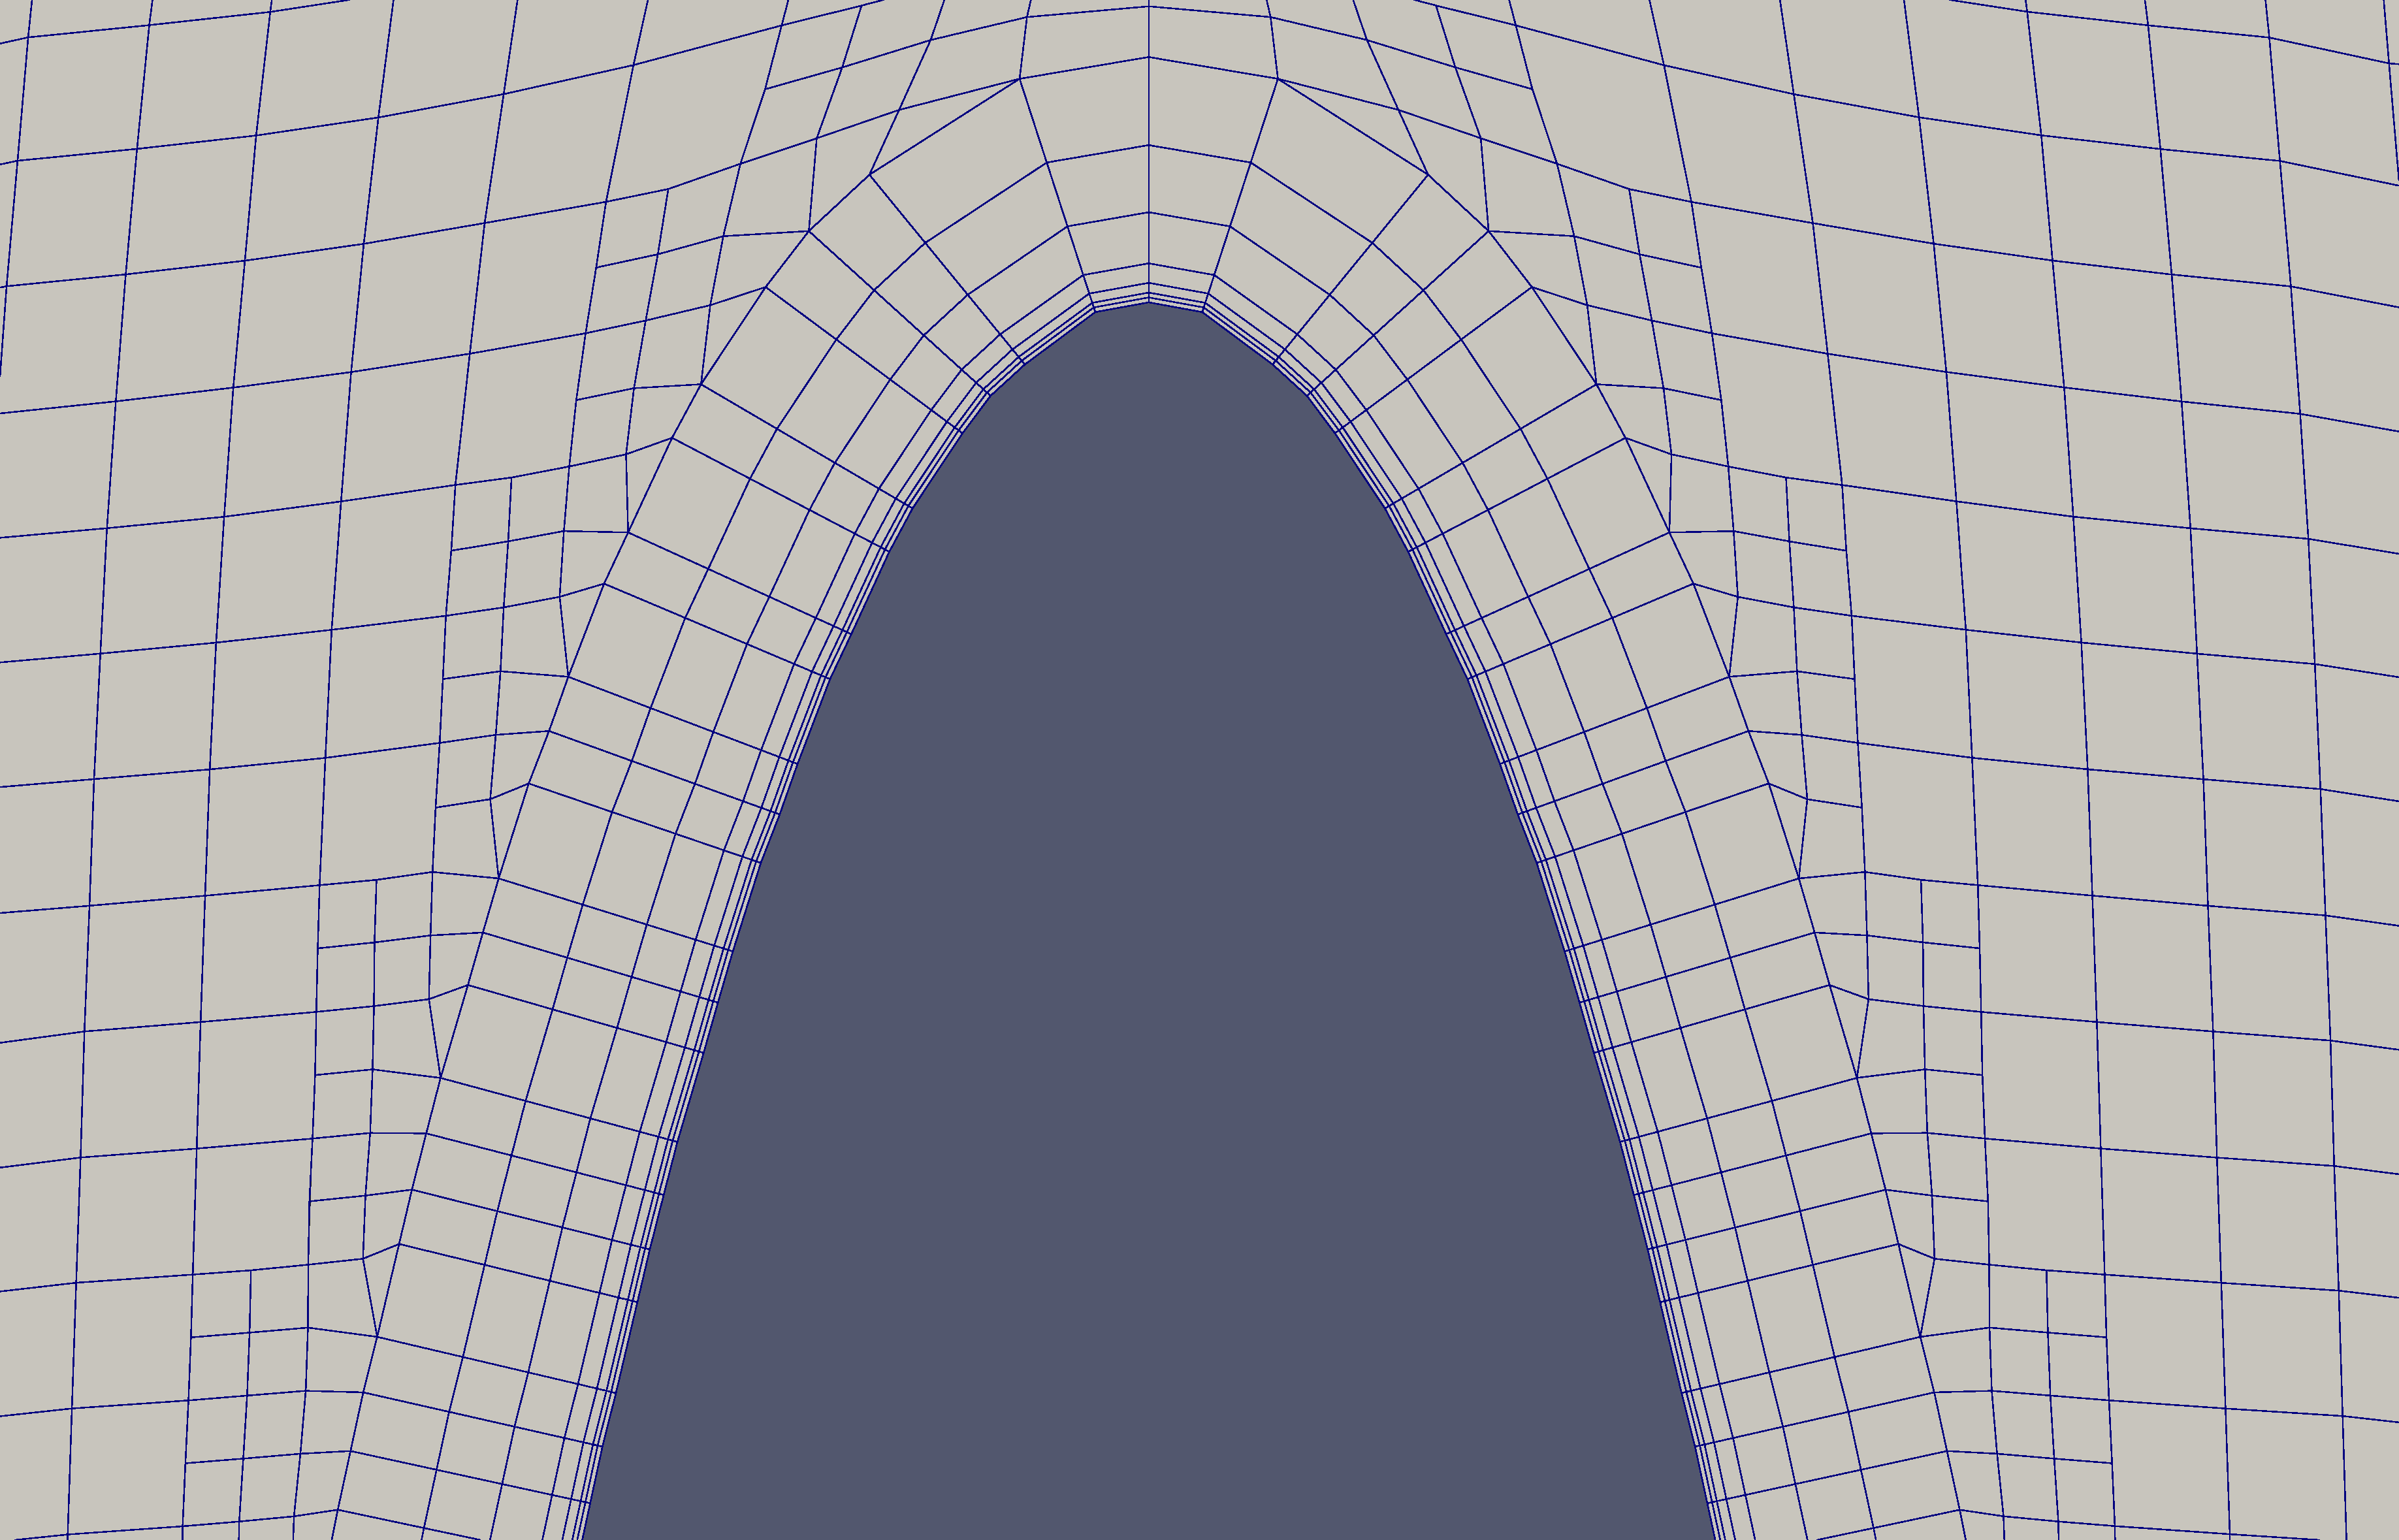
\includegraphics[width=5cm]{{images/mesh-120/view-bladetip-zoom}.pdf}
\end{figure}

\begin{figure}[H]
\centering
\includegraphics[width=4.5cm]{images/mesh-120/view-blade0.pdf}
\quad
\begin{tabular}[b]{lr}
\toprule
Cells                 & $113754$\\
Max Skewness          & $2.71645$\\
Max non-orthogonality & $58.52\,^{\circ}$\\
Max aspect ratio      & $16.1092$\\ \bottomrule
\end{tabular}
\end{figure}

\end{frame}


\section{Schemes}
%%%%%%%%%%%%%%%%%%%%%%%%%%%%%%%%%%%%%%%%%%%%%%
\begin{frame}
\frametitle{Numeric schemes - Time schemes}

Time schemes define the way in which a propriety is integrated in time. 
Depending on the choice of the user, an old $\phi^0$ or old-old $\phi^{00}$ solution will be required.

%\foam{backward} scheme is an implicit second order scheme, conditionally stable. 
%Since it does not diverge we take that as scheme for our complete simulation.

\begin{figure}[H]
\centering
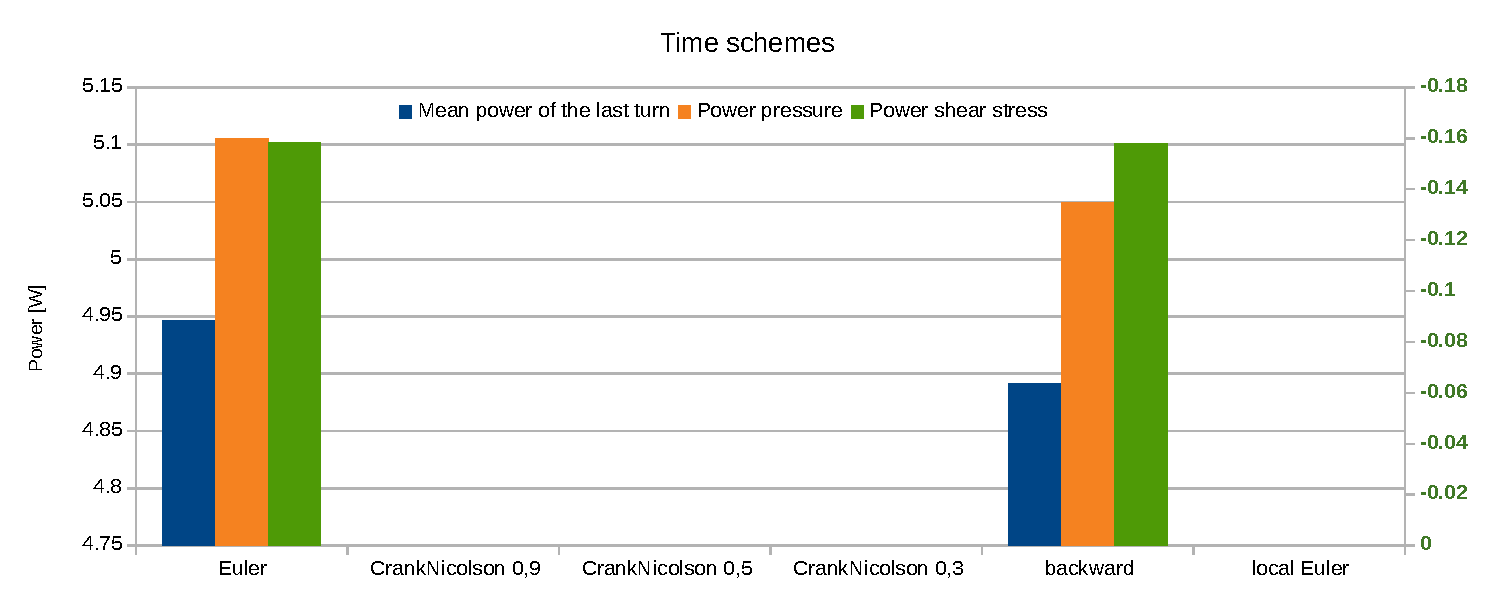
\includegraphics[width=\linewidth]{images/schemes/timeschems-results.pdf}
\end{figure}

\end{frame}


%%%%%%%%%%%%%%%%%%%%%%%%%%%%%%%%%%%%%%%%%%%%%%
\begin{frame}
\frametitle{Numeric schemes - Gradient schemes}
The gradient of a certain quantity $\phi$ rappresent the way in which that propriety is changing along a direction.

%\begin{equation}
%\nabla \phi = \begin{bmatrix} \frac{\partial \phi}{\partial x} \\ \frac{\partial \phi}{\partial y} \\\frac{\partial \phi}{\partial z}\end{bmatrix} 
%\end{equation}

\begin{figure}[H]
\centering
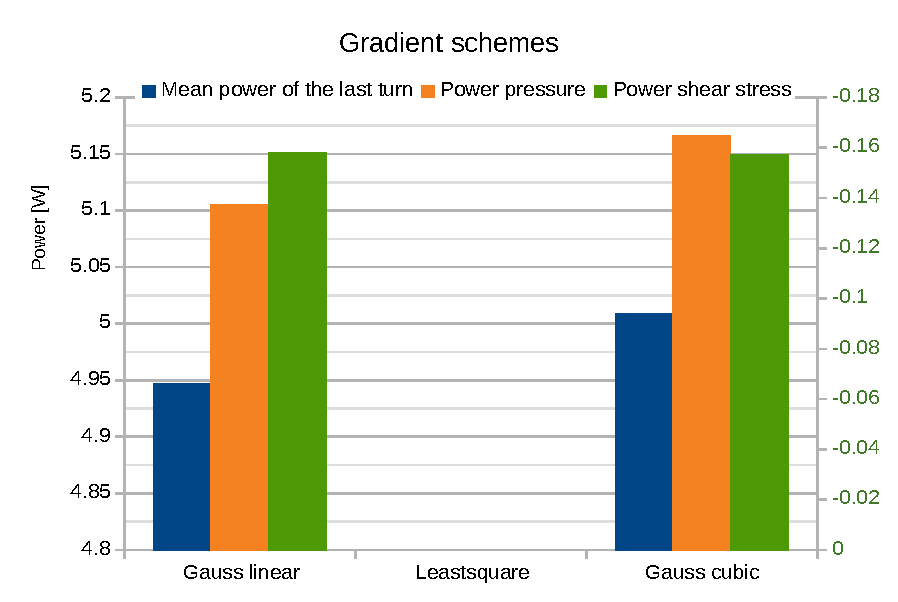
\includegraphics[width=10cm]{images/schemes/gradschems-results.pdf}
\end{figure}


\end{frame}




%%%%%%%%%%%%%%%%%%%%%%%%%%%%%%%%%%%%%%%%%%%%%%
\begin{frame}
\frametitle{Numeric schemes - Divergence schemes}
The divergence of a propriety $\bm{U}$ rappresent the rate at which that quantity is changing.

We are only testing divergence schemes of the velocity since it is in our opinion the most relevant quantity.

\begin{figure}[H]
\centering
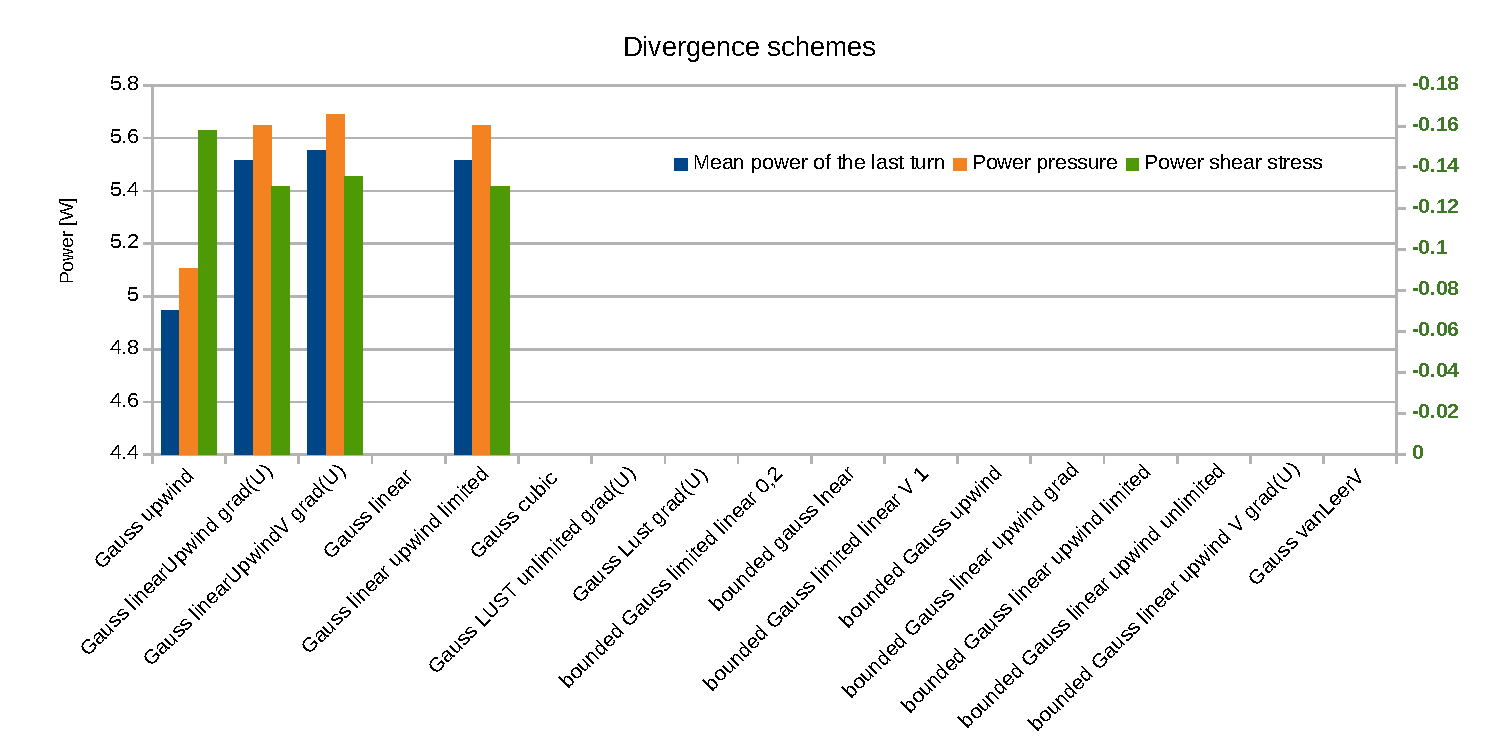
\includegraphics[width=\linewidth]{images/schemes/divschems-results.pdf}
\end{figure}


\end{frame}




%%%%%%%%%%%%%%%%%%%%%%%%%%%%%%%%%%%%%%%%%%%%%%
\begin{frame}
\frametitle{Numeric schemes - Laplacian schemes}

Laplacian typically it is associated to the diffusive term. 
\\
Gauss scheme is the only one available and requires the interpolation scheme used and the normal gradient scheme, defined in the proper subsection \textit{interpolationSchemes} and \textit{snGradSchemes}.
\begin{figure}[H]
\centering
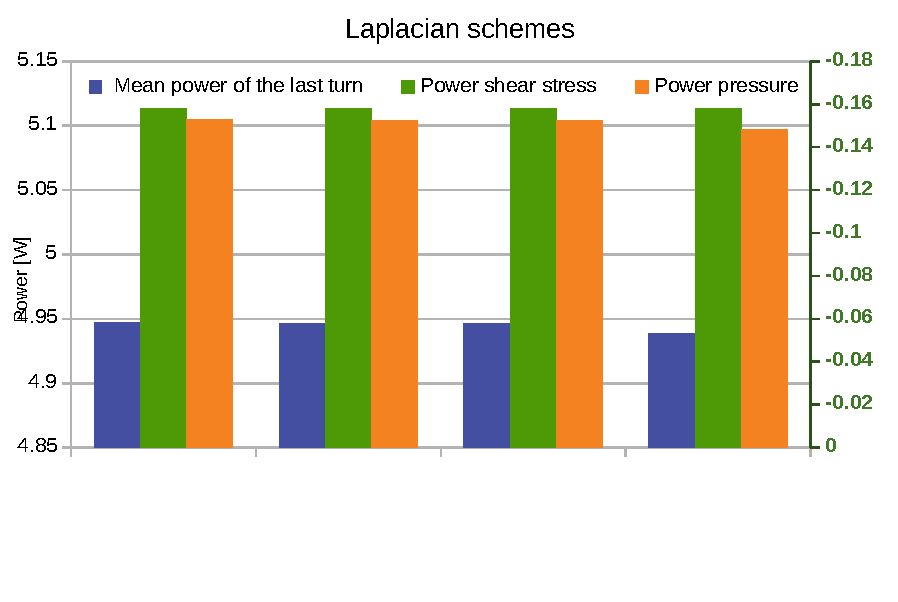
\includegraphics[width=10cm]{images/schemes/laplacianschems-results.pdf}
\end{figure}
\end{frame}



%%%%%%%%%%%%%%%%%%%%%%%%%%%%%%%%%%%%%%%%%%%%%%
\begin{frame}
\frametitle{Numeric schemes - Conclusions}
Finally we have chosen the following schemes:
\begin{figure}[H]
\begin{tabular}{ll} 
\foam{time} \quad \quad & \foam{backward} \\ 
\foam{divergence} \quad \quad & \foam{Gauss upwind} \\
\foam{laplacian} \quad \quad &\foam{Gauss linear corrected} \\ 
\foam{grad}  \quad \quad & \foam{Gauss cubic} 
\end{tabular}
\end{figure}

\begin{figure}[H]
\centering
\subfigure[Reference case]{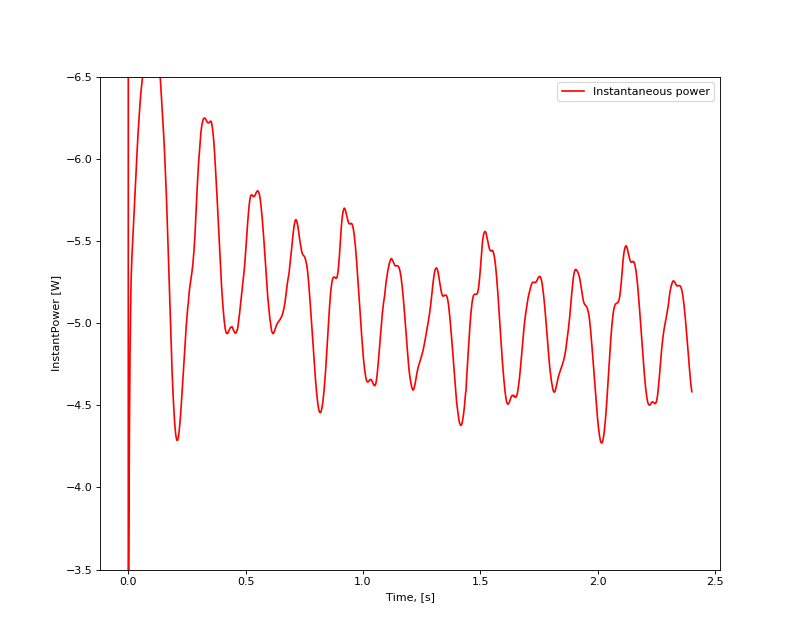
\includegraphics[width=3.5cm]{{images/schemes/InstantPower_casobase}.png}}
\subfigure[Backward]{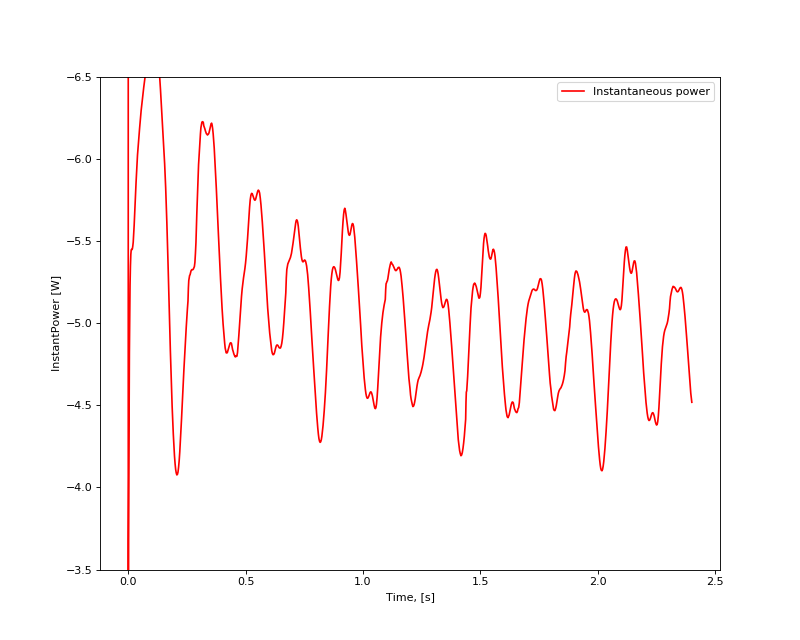
\includegraphics[width=3.5cm]{{images/schemes/InstantPower_backward}.png}}
\subfigure[Linear upwind]{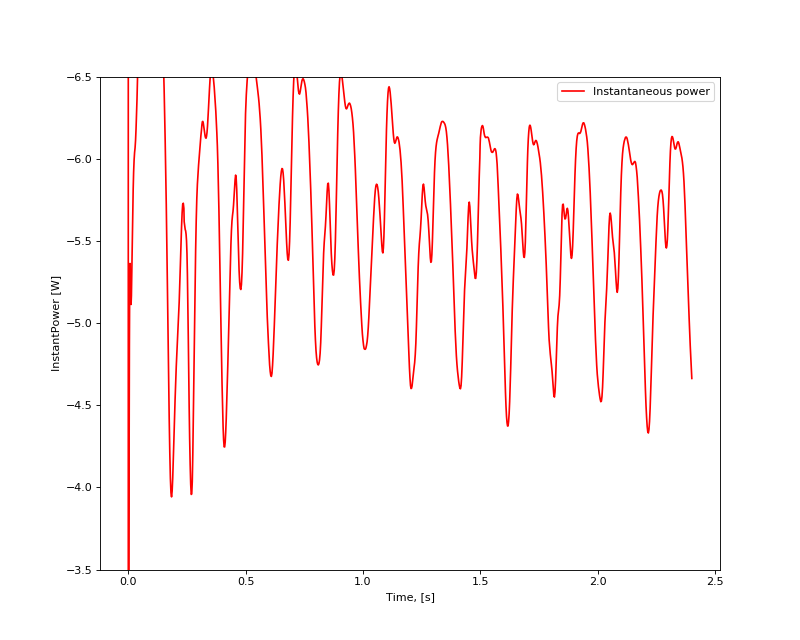
\includegraphics[width=3.5cm]{{images/schemes/InstantPower_linearupwind}.png}}
%\caption{Instantaneous power with difference schemes.}
%\label{fig:schemes-instant-power}
\end{figure}

\end{frame}



\section{Solver parameters}



%%%%%%%%%%%%%%%%%%%%%%%%%%%%%%%%%%%%%%%%%%%%%%
\begin{frame}
\frametitle{Solver parameters}

Starting from in the in-class base setup, the analysis of the residuals highlights that the pressure was the most problematic quantity in terms of convergence.

To improve the results we can deal with:
\begin{itemize}
\item[$\cdot$] outer correctors;
\item[$\cdot$] inner correctors;
\item[$\cdot$] non-orthogonal correctors;
\item[$\cdot$] Courant number.
\end{itemize}

The default schemes are:
\begin{itemize}
\item[$\cdot$] \foam{PIMPLE}: 50 outers, 1 inner;
\item[$\cdot$] \foam{PISO}: 1 outer, 2 inner.
\end{itemize}

Since we want to reduce pressure residuals we have tested a different version of standard \foam{PISO}:
\begin{center}
\foam{PISO}: 1 outer, 20 inner.
\end{center}

%\begin{figure}[H]
%\centering
%\subfigure[Pimple 50 outer 1 inner]{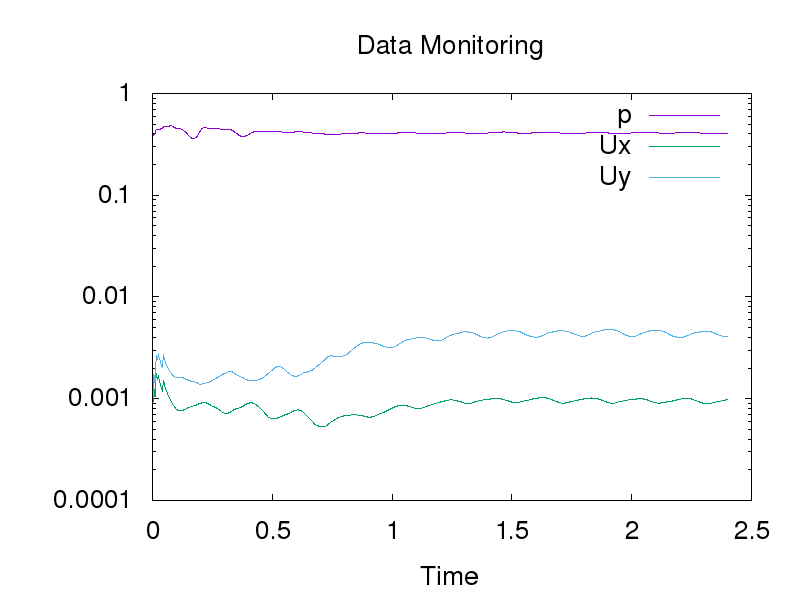
\includegraphics[width=5cm]{{images/solver/residuals50-1}.png}}
%\subfigure[Piso 1 outer 20 inner]{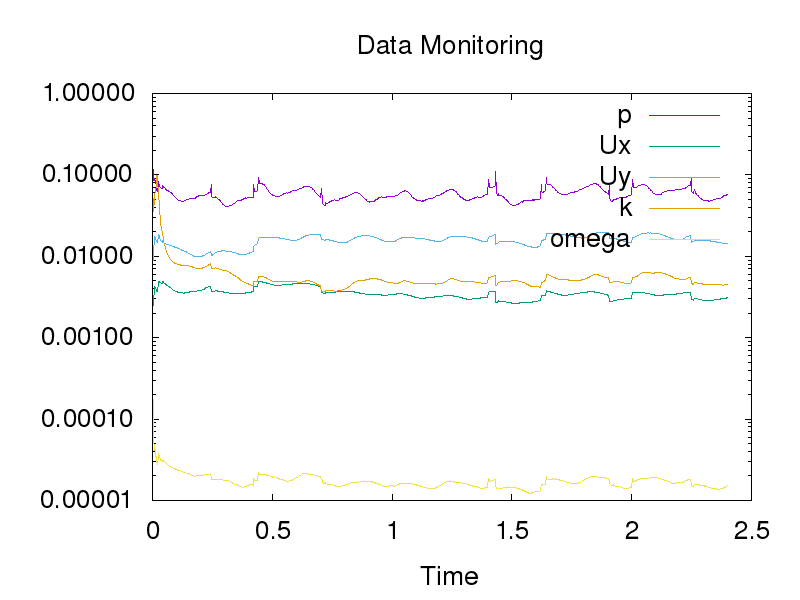
\includegraphics[width=5cm]{{images/solver/residuals1-20}.png}}
%\caption{Residuals comparison bewteen standard Pimple and our Piso.}
%\label{fig:solver-residuals-bad}
%\end{figure}

\end{frame}


%%%%%%%%%%%%%%%%%%%%%%%%%%%%%%%%%%%%%%%%%%%%%%
\begin{frame}
\frametitle{Solver parameters}

This modified version of the \foam{PISO} allows us to increase the Courant up to 50
without comprimizing pressure residuals, but with a gain of $\approx 10$ times in terms of computational cost.

\begin{figure}[H]
\centering
\subfigure[Pimple 50 outer 1 inner]{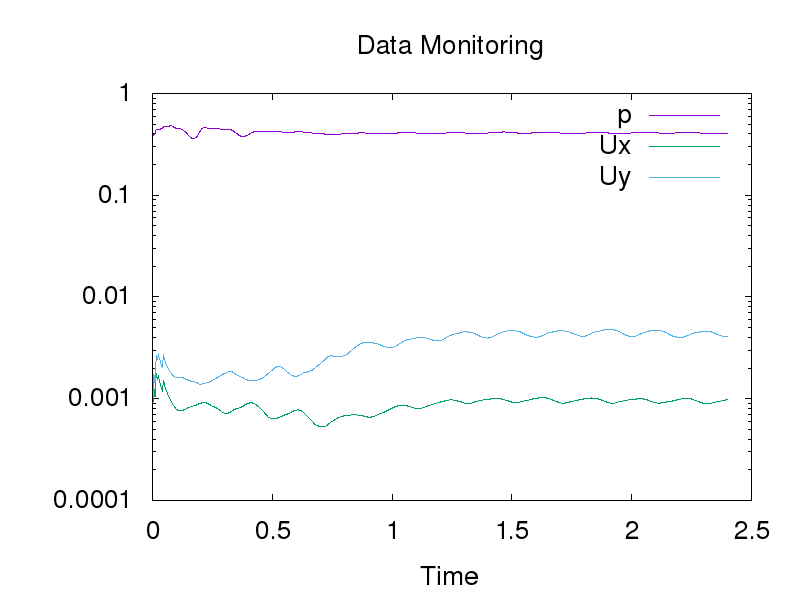
\includegraphics[width=5cm]{{images/solver/residuals50-1}.png}}
\subfigure[Piso 1 outer 20 inner]{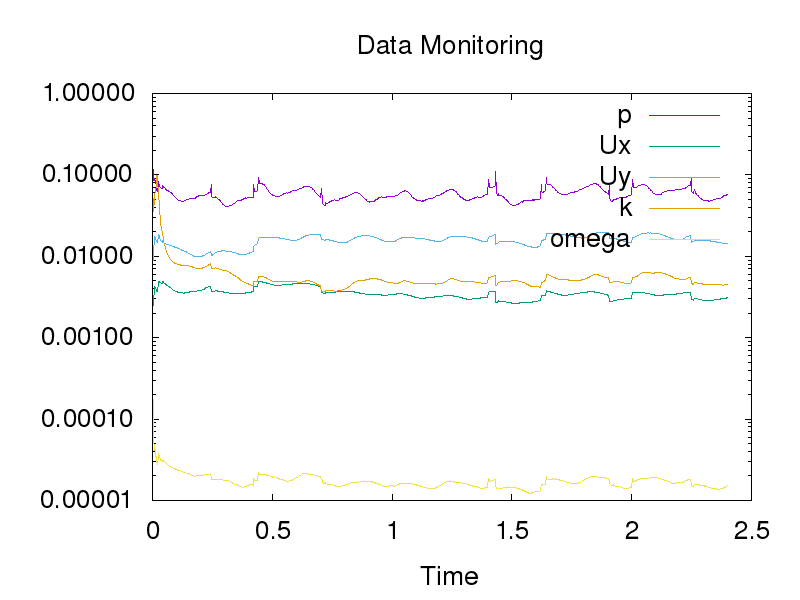
\includegraphics[width=5cm]{{images/solver/residuals1-20}.png}}
%\caption{Residuals comparison bewteen standard Pimple and our Piso.}
%\label{fig:solver-residuals-bad}
\end{figure}

\end{frame}



\section{Turbolence}


%%%%%%%%%%%%%%%%%%%%%%%%%%%%%%%%%%%%%%%%%%%%%%
\begin{frame}
\frametitle{Turbolence}

Turbolence model adopted in base case was \kepsilon.

By further investigation on mesh 120 it was highlighted that $y^+$ was not suitable for such grid-model combination.

\begin{table}[H]
\centering
\begin{tabular}{rcc}
\toprule
           & min $y^+ $          & max $y^+$  \\ \midrule
lower wall & $\round{6.793848e-01}$         & $\round{4.095234e+00}$ \\
blade0     & $\round{5.503802e-02}$ & $\round{7.997351e-01}$ \\
blade1     & $\round{4.869300e-02}$         & $\round{1.742530e-01}$ \\
blade2     & $\round{7.257931e-02}$         & $\round{7.748824e-01}$ \\ \bottomrule
\end{tabular}
%\caption{Min and max $y^+$ values on the walls}
%\label{table:turbolence-yplus}
\end{table}

Moreover we also expect to have flow detachment and recirculation because of the wide range in incidence angle.

\end{frame}



%%%%%%%%%%%%%%%%%%%%%%%%%%%%%%%%%%%%%%%%%%%%%%
\begin{frame}
\frametitle{Turbolence}
We will move to models which solve the boundary layer instead of applying wall functions to mimic the phenomenon in a better way (\komegasst).

Since in turbomachinery is common the use of \komegasst we compare it to less appropriate \kepsilon and laminar.


\begin{figure}[H]
\centering
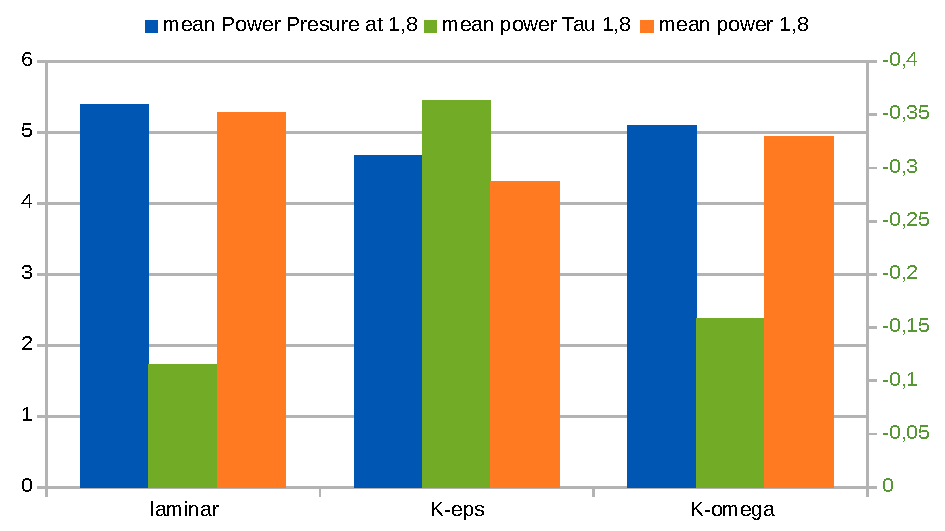
\includegraphics[width=8cm]{images/turbulence/MeanPower_comparison-detailed.pdf} 
%\caption{Power comparison}
%\label{fig:turbolence-powercomparison}
\centering
\end{figure}

\end{frame}


%%%%%%%%%%%%%%%%%%%%%%%%%%%%%%%%%%%%%%%%%%%%%%
\begin{frame}
\frametitle{Turbolence}

\kepsilon model underestimate the pressure power and overestimate the shear power.
\quad $\Rightarrow$ Resulting power double penalized.

Probably the wall functions are not able to fit correctly boundary layers in all their shadings (detachment, flow recirculation, ...).

\begin{figure}
\centering
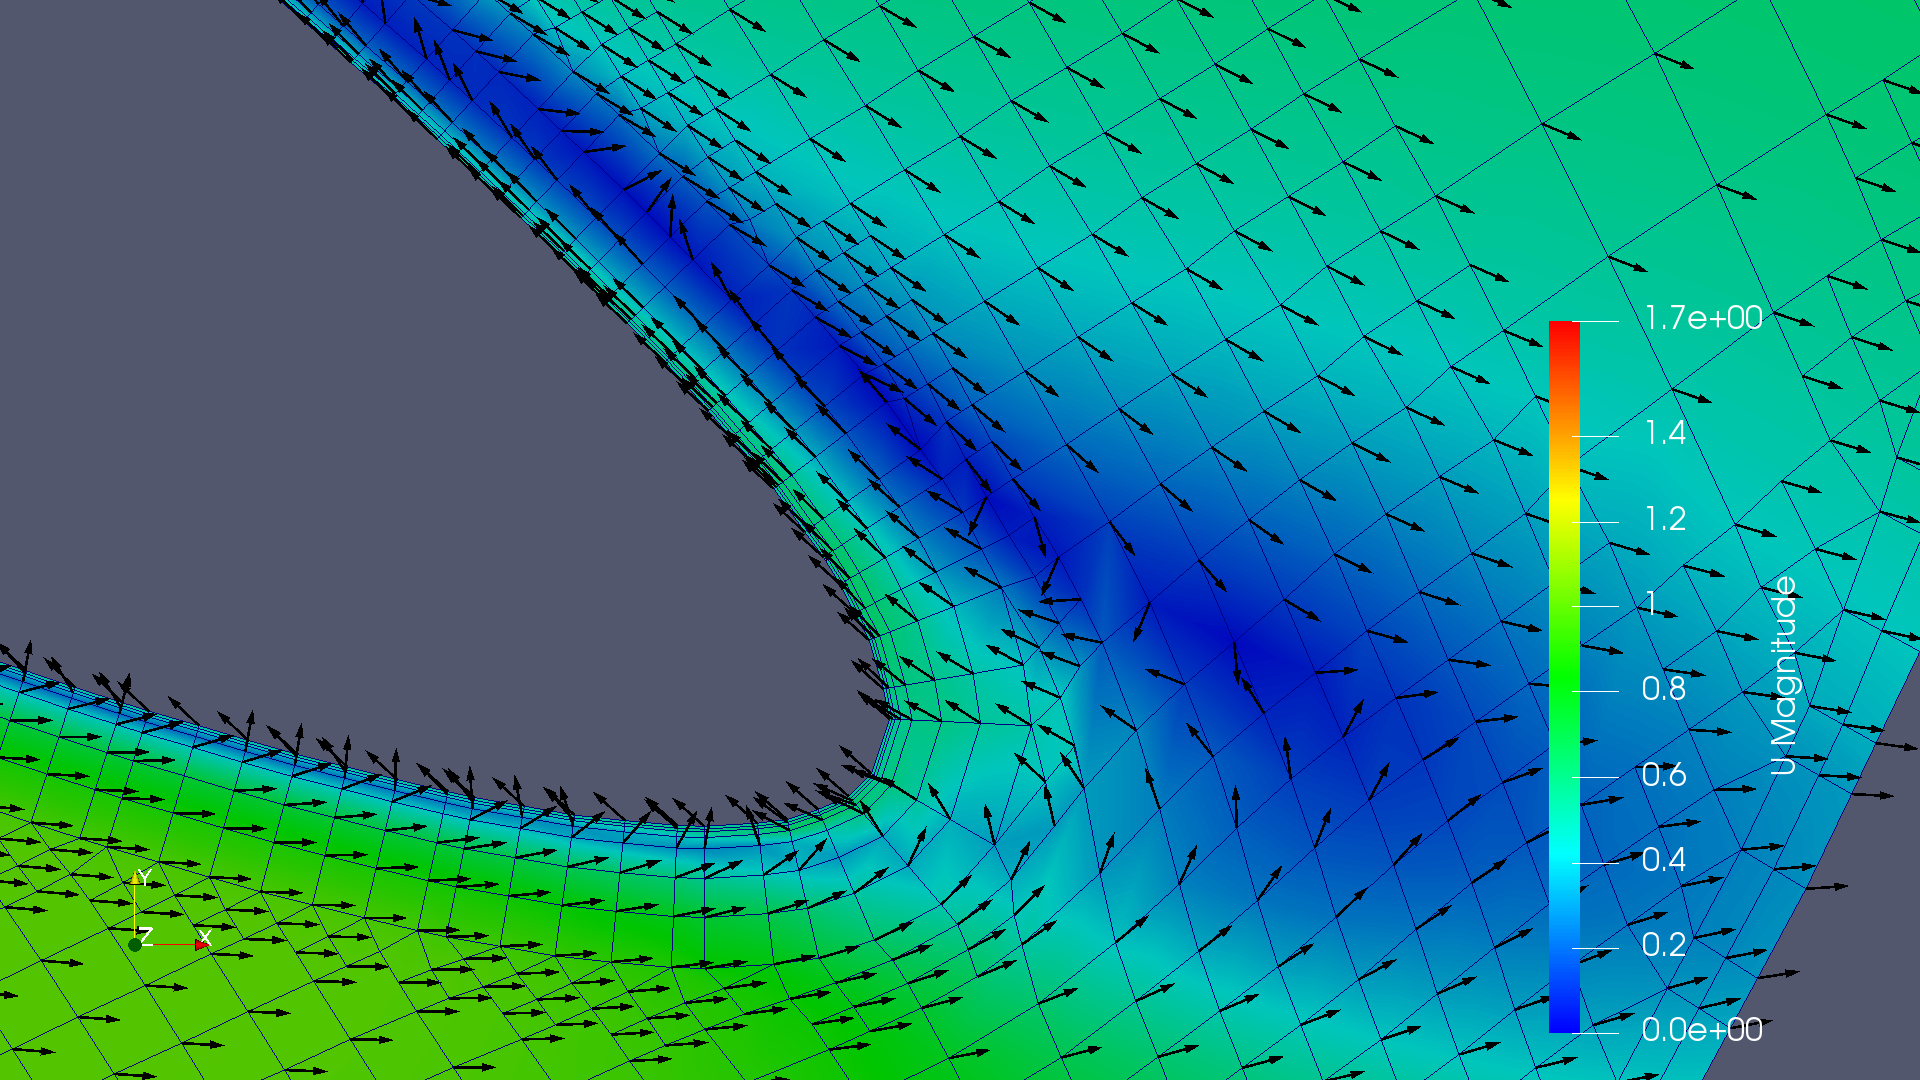
\includegraphics[width=8cm]{images/turbulence/recirculation_scalarScaledMESH.png}
\end{figure}
\end{frame}


%%%%%%%%%%%%%%%%%%%%%%%%%%%%%%%%%%%%%%%%%%%%%%
\begin{frame}
\frametitle{Turbolence - boundary layer}

The resulting trend of the velocity $U^+$ inside the boundary layer with \komegasst model reveals the typical regions of the theoretical analysis of the plane plate:
\begin{itemize}
\item[$\cdot$] linear for $y^+ < 10$;
\item[$\cdot$] buffer for $10 < y^+ < 30$;
\item[$\cdot$] logarithmic for $y^+ > 30$;
\end{itemize}

\begin{figure}
\centering
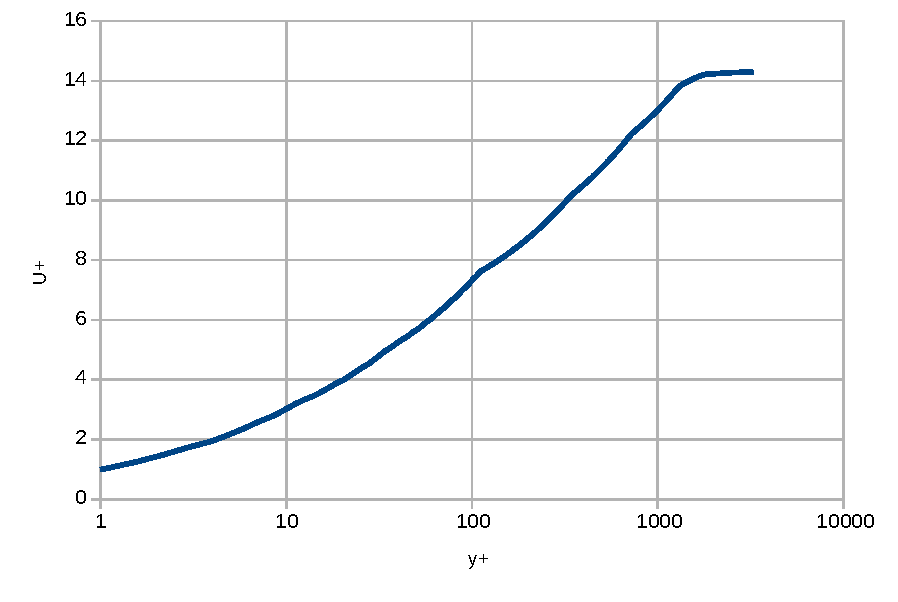
\includegraphics[width=7cm]{images/turbulence/boundarylayer.pdf}
\end{figure}

\end{frame}



%%%%%%%%%%%%%%%%%%%%%%%%%%%%%%%%%%%%%%%%%%%%%%
\begin{frame}
\frametitle{Turbolence intensity}

Up to now we have performed all simulations with $5\%$ turbolent intensity.
How about changing the value? 

To reply to this answer we have once more implemented a sensibility analysis based on the variation of turbolent intensity.

We range from a very moderate up to a quite intense turbolence.


\begin{figure}[H]
\centering
%\caption{Power comparison}
\subfigure[Total power.]{\includegraphics[width=5cm]{{images/turbolentsensitivity/power}.pdf}}
\quad
\subfigure[Normal and tangential power.]{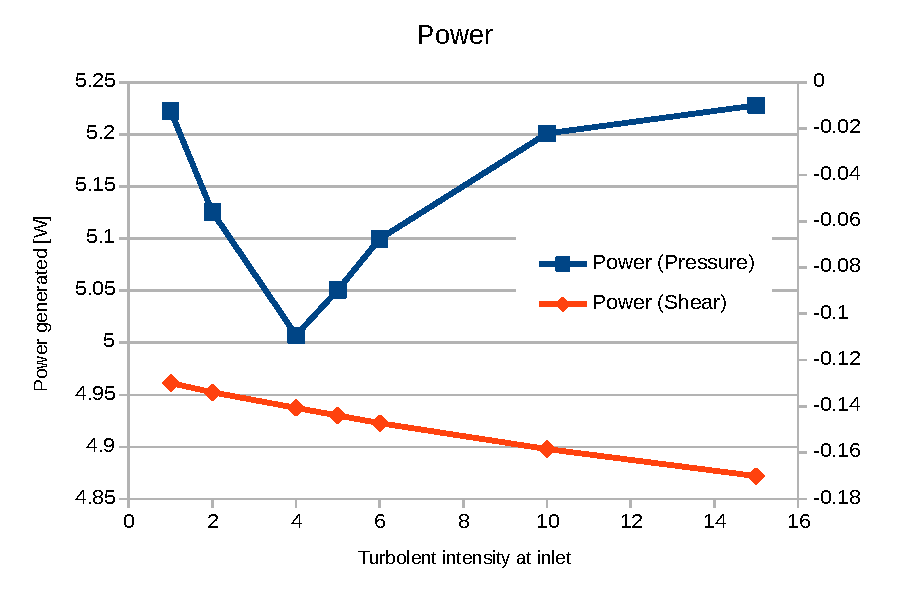
\includegraphics[width=5cm]{{images/turbolentsensitivity/power-ptau}.pdf}}
%\label{fig:turbintensity-power}
\end{figure}

\end{frame}


\section{Extended domain}




%%%%%%%%%%%%%%%%%%%%%%%%%%%%%%%%%%%%%%%%%%%%%%
\begin{frame}
\frametitle{Extended domain}
Looking at our symulation we can clearly see that before and after the turbine, the flow has not
reach yet an unperturbed motion. 
And since there is the possibility that boundary will affect our
solution, we run the reference case with different domain length.

\begin{figure}[H]
\centering
\includegraphics[width=8cm]{images/longmesh/confronto_mesh_long.png}
%\caption{Representation of different meshes tested.}
\end{figure}

\end{frame}



%%%%%%%%%%%%%%%%%%%%%%%%%%%%%%%%%%%%%%%%%%%%%%
\begin{frame}
\frametitle{Extended domain}

Starting point is the case where the mesh is limited between $-0.6\m$ to  $0.6\m$. 
Then different meshes
were tested increasing dimension in symmetric way, to take into account the pressure rise effect
at the bottom of the channel as well as the wake and mixing downstream.

\begin{figure}[H]
\centering
\includegraphics[width=8cm]{images/longmesh/power.pdf}
%\caption{Residuals of gravity simulation.}
%\label{fig:domainlong-power}
\end{figure}

\end{frame}


\section{Boundaries and gravity}


%%%%%%%%%%%%%%%%%%%%%%%%%%%%%%%%%%%%%%%%%%%%%%
\begin{frame}
\frametitle{Gravity effect and enhanced boundary conditions}

To correct rappresent the problem our idea is to consider also gravitational effect. 
However before doing so we need to modify boundary conditions.

\begin{itemize}
\item[$\cdot$] \textbf{Velocity}: change on the upper wall from \foam{slip} to \foam{freestreem}

\item[$\cdot$] \textbf{Pressure}: change on outlet from uniformly fixed to $0 \,\text{m}^2/\text{s}^2$ to \foam{zeroGradient}. 
This is the crucial B.C. that allows us to implement gravitational effect.

\item[$\cdot$] \textbf{Turbolent kinetic energy}: change on initial condition (not B.C.) to  $ 3/2 \cdot \left(I\, \text{U} \right) ^2 = 0.00375 \m^2 / \s^2$.
the upper wall is set to \foam{freestreem}.

\item[$\cdot$] \textbf{Turbolent kinematic viscosity}: change only on initial condition to $0.000335$ to try to speed up regime convergence.
\end{itemize}

%\textbf{Velocity} \quad change on the upper wall from \foam{slip} to \foam{freestreem}
%\\
%\textbf{Pressure} \quad change on outlet from uniformly fixed to $0 \,\text{m}^2/\text{s}^2$ to \foam{zeroGradient}. 
%This is the crucial B.C. that allows us to implement gravitational effect.
%\\
%\textbf{Turbolent kinetic energy} \quad change on initial condition (not B.C.) to  $ 3/2 \cdot \left(I\, \text{U} \right) ^2 = 0.00375 \m^2 / \s^2$.
%the upper wall is set to \foam{freestreem}.
%\\
%\textbf{Turbolent kinematic viscosity} change only on initial condition to $0.000335$ to try to speed up regime convergence.
\end{frame}



%%%%%%%%%%%%%%%%%%%%%%%%%%%%%%%%%%%%%%%%%%%%%%
\begin{frame}
\frametitle{Enhanced boundary conditions}

\begin{figure}[H]
\centering
\subfigure[Pressure]{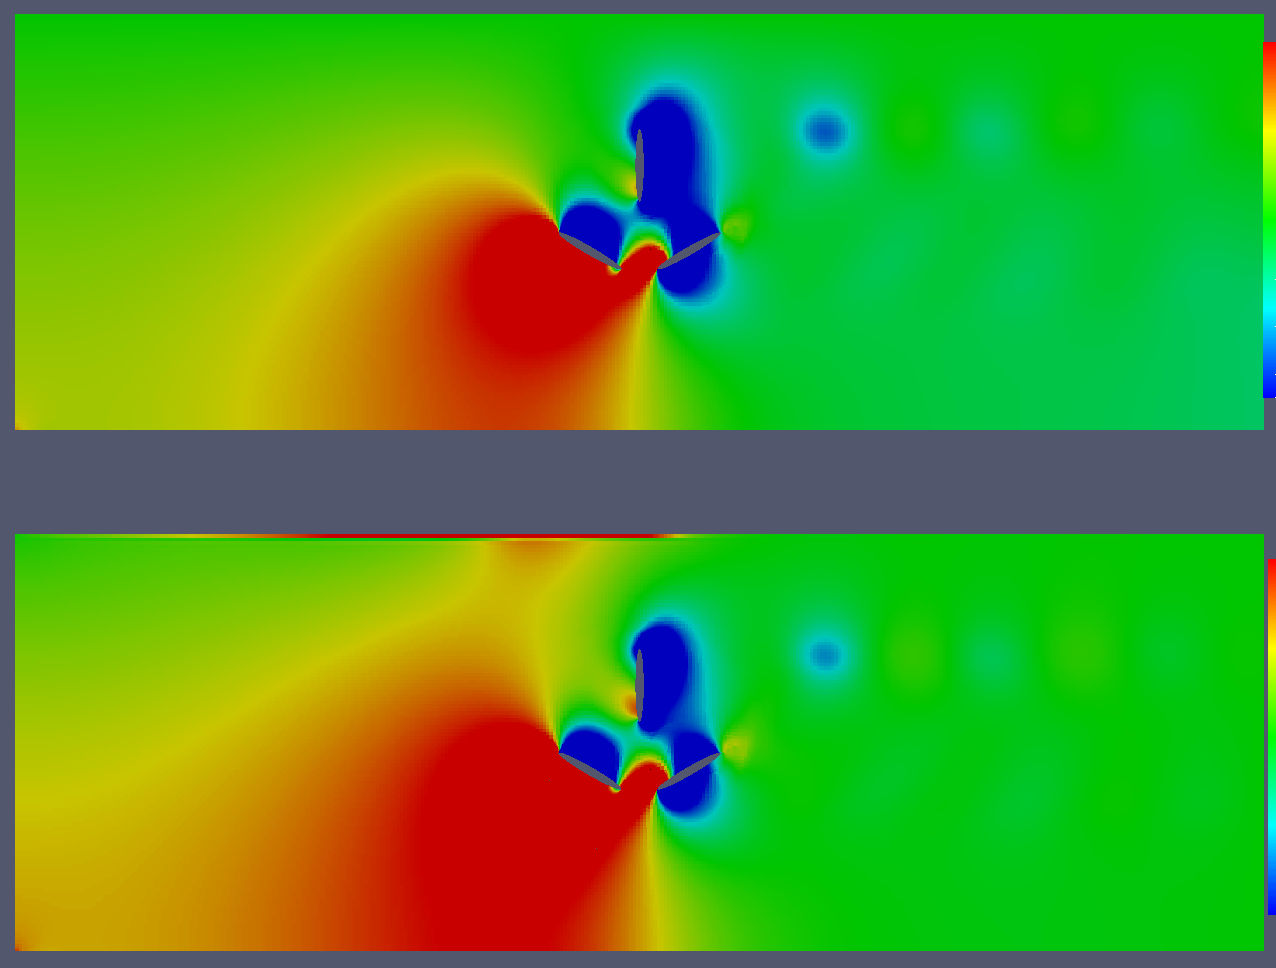
\includegraphics[height=3.5cm]{{images/gravity/boundaries-p}.png}}
\quad
\subfigure[Turbolent Kinetic energy]{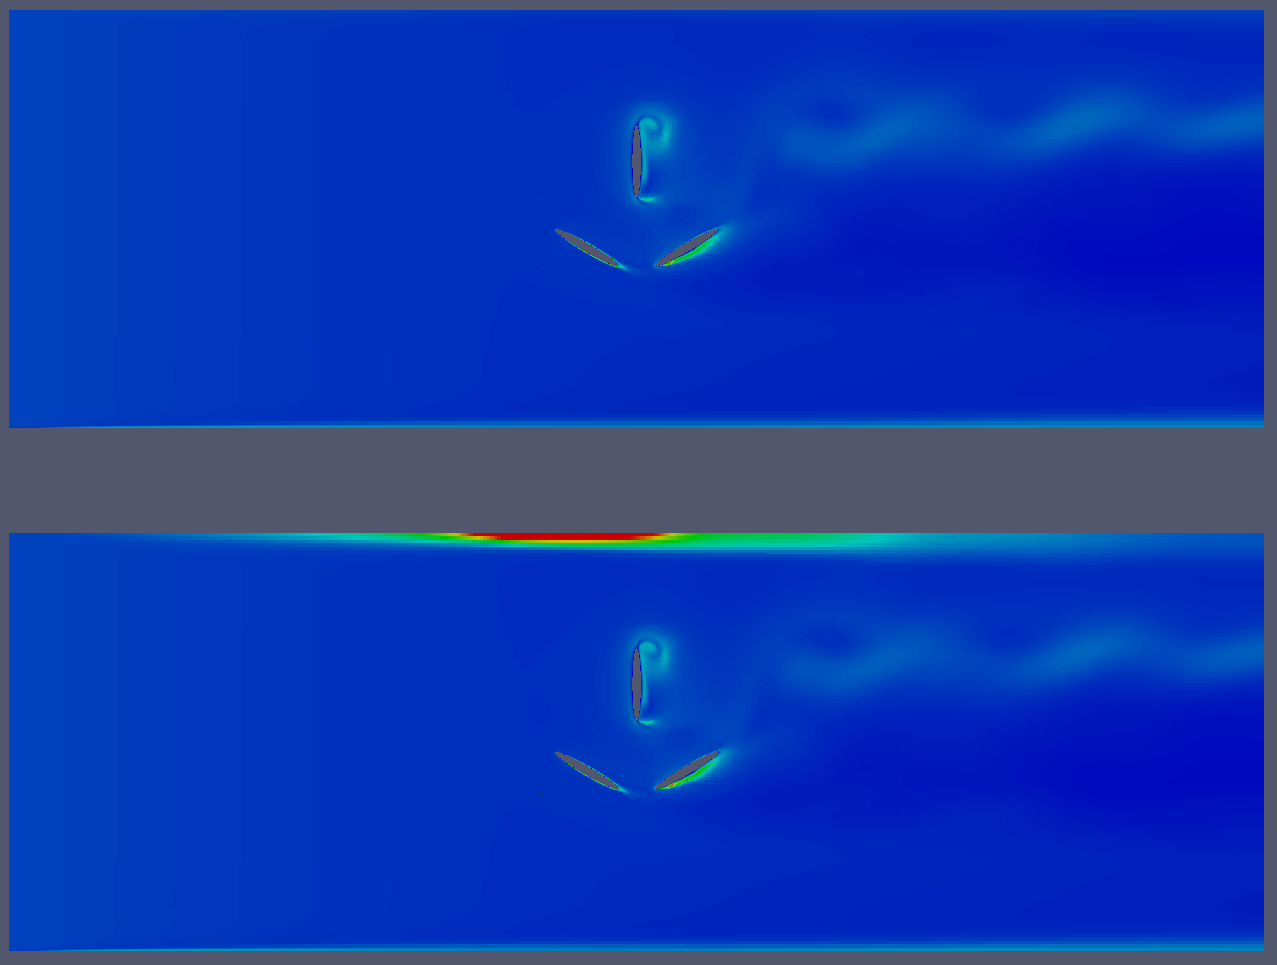
\includegraphics[height=3.5cm]{{images/gravity/boundaries-k}.png}}
%\caption{Pressure and Turbolent kinetic energy fields at time 2.4 seconds}
%\label{fig:gravity-trends}
\end{figure}

\vspace{-0.3cm}
\begin{table}[H]
\centering
\tiny
\begin{tabular}{lrr}
\toprule
								   & Default boundaries        & Enhanced boundaries       \\ \midrule
Power [W]                          & $\round{4.94689061527}$   & $\round{5.02917144498}$   \\
Power (pressure) [W]               & $\round{5.10506073361}$   & $\round{5.18583998598}$   \\
Power(Shear stress)  [W]           & $\round{-0.158170118337}$ & $\round{-0.156668541001}$ \\
Total pressure inlet (2.4 s) [Pa]  & $\round{0.6503034*1000}$  & $\round{0.6320083*1000}$  \\
Total pressure outlet (2.4 s) [Pa] & $\round{0.4826165*1000}$  & $\round{0.4425995*1000}$  \\
Total pressure drop (2.4 s) [Pa]   & $\round{167.6869}$        & $\round{189.4088}$        \\ \bottomrule
\end{tabular}
\end{table}
\end{frame}



%%%%%%%%%%%%%%%%%%%%%%%%%%%%%%%%%%%%%%%%%%%%%%
\begin{frame}
\frametitle{Gravitational effect}
Even if gravitational force completes our model, there is no significant impact on the final results.

\begin{figure}[H]
\centering
\subfigure{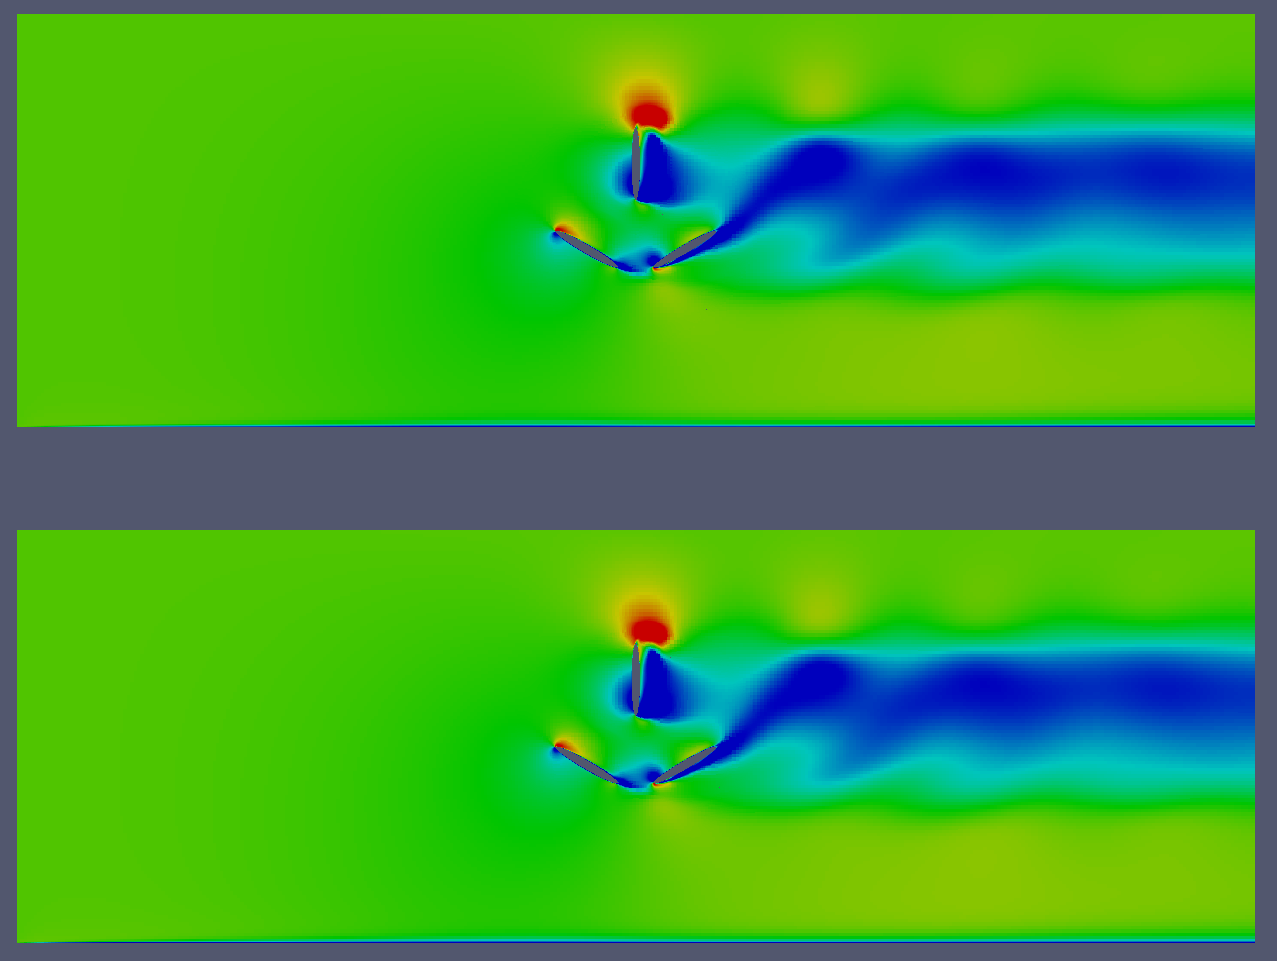
\includegraphics[height=3.5cm]{{images/gravity/U-2.4}.png}}
\quad
\subfigure{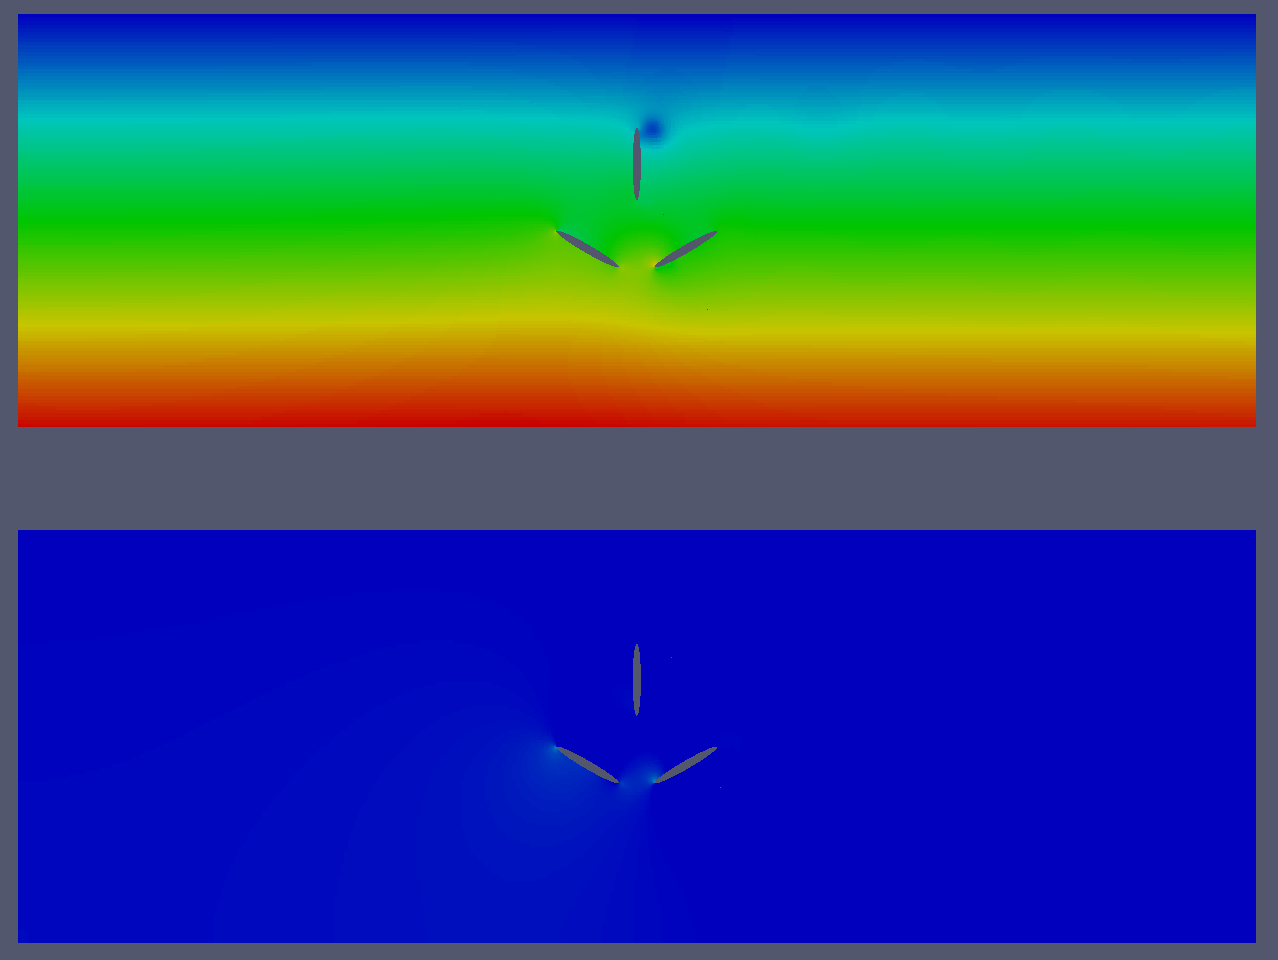
\includegraphics[height=3.5cm]{{images/gravity/p-2.4}.png}}
%\caption{Pressure and Velocity fields at time 2.4 seconds}
%\label{fig:gravity-fields}
\end{figure}

\vspace{-0.5cm}
\begin{table}[H]
\centering
\tiny
\begin{tabular}{lrr}
\toprule
                                   & Gravity enabled           & Gravity disabled          \\ \midrule
Power [W]                          & $\round{5.02801934555}$   & $\round{5.02917144498}$   \\
Power (pressure) [W]               & $\round{5.18466414042}$   & $\round{5.18583998598}$   \\
Power(Shear stress) [W]            & $\round{-0.156644794865}$ & $\round{-0.156668541001}$ \\
Total pressure inlet (2.4 s) [Pa]  & $\round{3059.583}$        & $\round{632.0083}$        \\
Total pressure outlet (2.4 s) [Pa] & $\round{2870.286}$        & $\round{442.5995}$        \\
Total pressure drop (2.4 s) [Pa]   & $\round{189.297}$         & $\round{189.4088}$        \\ \bottomrule
\end{tabular}
%\caption{Comparison with and without gravity}
%\label{table:gravity-comparison}
\end{table}
\end{frame}


%%%%%%%%%%%%%%%%%%%%%%%%%%%%%%%%%%%%%%%%%%%%%%
\begin{frame}
\frametitle{Gravitational effect - residuals}

Even if the contribution of both the new B.C. and the gravity seems quite negligible,
a positive effect can be noticed looking at the residuals trend.

\vspace{-0.15cm}
\begin{figure}[H]
\centering
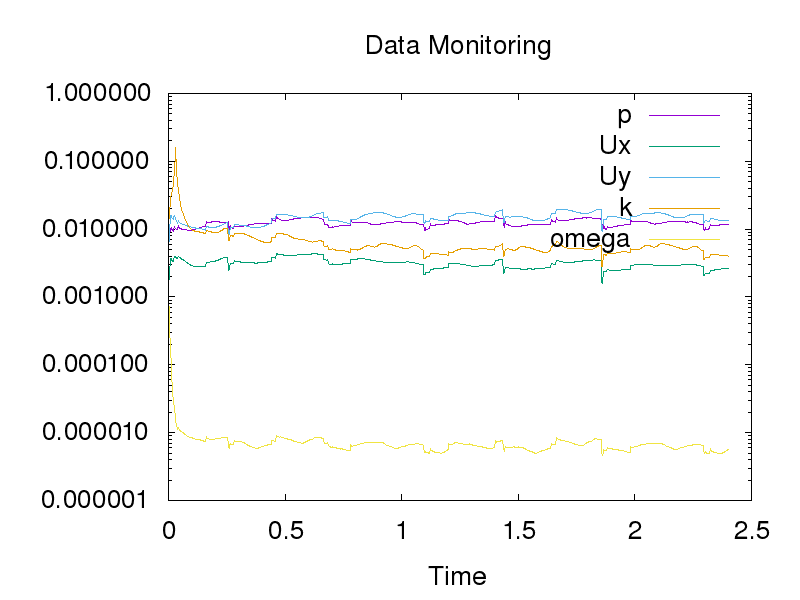
\includegraphics[width=9cm]{images/gravity/residuals.png}
%\caption{Residuals of gravity simulation.}
\end{figure}

\end{frame}



%%%%%%%%%%%%%%%%%%%%%%%%%%%%%%%%%%%%%%%%%%%%%%
\begin{frame}
\frametitle{Gravitational effect - extended domain}

To conclude the grativitational field analysis, we have performed few simulations with extended
domain. We have tried to both extends upstream, downstream and in a symmetric way the total
domain.

\begin{figure}[H]
\centering
\includegraphics[width=10cm]{images/gravity/{U-extended}.png}
%\caption{Velocity field representation of all the domains.}
%\label{fig:gravity-extendeddomain}
\end{figure}

\end{frame}


%%%%%%%%%%%%%%%%%%%%%%%%%%%%%%%%%%%%%%%%%%%%%%
\begin{frame}
\frametitle{Gravitational effect - extended domain}

It is interesting to notice that only upstream region has an influence on the power.

\begin{table}[H]
\tiny
\centering
\begin{tabular}{lrrr}
\toprule
                           & Power [W]               & Power (pressure) [W]    & Power(Shear stress) [W]   \\ \midrule
Gravity enabled            & $\round{5.02801934555}$ & $\round{5.18466414042}$ & $\round{-0.156644794865}$ \\
Gravity disabled           & $\round{5.02917144498}$ & $\round{5.18583998598}$ & $\round{-0.156668541001}$ \\
Gravity (2.4 m symmetric)  & $\round{4.64901900925}$ & $\round{4.80320537572}$ & $\round{-0.154186366469}$  \\
Gravity (2.4 m downstream) & $\round{5.03340003987}$ & $\round{5.19009079263}$ & $\round{-0.156690752765}$ \\
Gravity (2.4 m upstream)   & $\round{4.61611451955}$ & $\round{4.76833335025}$ & $\round{-0.152218830708}$ \\
Gravity (3.6 m symmetric)  & $\round{4.6274730287}$  & $\round{4.77976509963}$ & $\round{-0.152292070926}$ \\ \bottomrule
\end{tabular}
%\caption{Extended domain comparison}
%\label{table:gravity-extended}
\end{table}
\vspace{-0.75cm}
\begin{figure}[H]
\centering
\includegraphics[width=5cm]{images/gravity/{power-extended}.pdf}
\includegraphics[width=5cm]{images/gravity/{U-0.6m-extended}.pdf}
%\caption{Power evolution with symmetric domains.}
%\label{fig:gravity-extended-power}
\end{figure}

%\begin{figure}[H]
%\centering
%\includegraphics[width=10cm]{images/gravity/{U-0.6m-extended}.pdf}
%\caption{Velocity distribution along y direction at x coordinate $0.6\m$.}
%\label{fig:gravity-U0.6-extended}
%\end{figure}

\end{frame}


\section{Blade Speed Ratio}

%%%%%%%%%%%%%%%%%%%%%%%%%%%%%%%%%%%%%%%%%%%%%%
\begin{frame}
\frametitle{Blade speed ratio}

From mesh sensitivity analysis, the power is quite accurately computed even
for a mesh size smaller that that we consider mesh independent.
To obtain more points we have decided to run most of the simulation with a mesh 80 instead  of 120.
Cells number is reduced from 110K to 60K. 


\begin{figure}[hbtp]
\centering
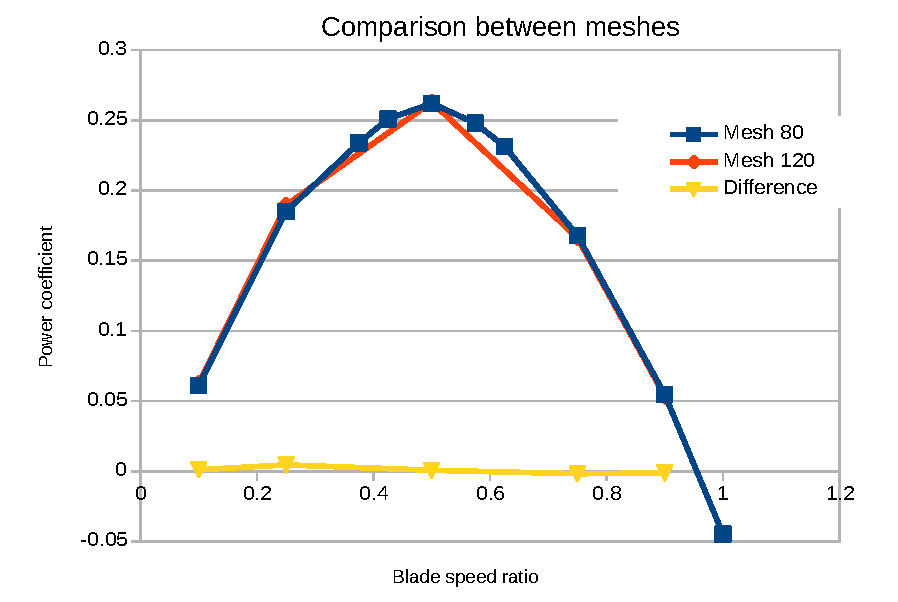
\includegraphics[width=8cm]{images/bsr/bsr-mesh80-120.pdf}
%\caption{Comparison between mesh 80 and mesh 120}
%\label{fig:bsr-comparison-80-120}
\end{figure}

\end{frame}


%%%%%%%%%%%%%%%%%%%%%%%%%%%%%%%%%%%%%%%%%%%%%%
\begin{frame}
\frametitle{Blade speed ratio}

For the calculation of the power coefficient we have considered as reference area:
$\text{A}_\text{reference} = 2\, \text{R} \cdot t = 0.0396 \msquare $
\begin{conditions}
R & 0.09 \m  \text{ distance between center of rotation and blade tip} \\
t & 0.22 \m \text{ is blade thickness}
\end{conditions}

\begin{table}[H]
\tiny
\centering
%\caption{Blade speed ratio results with mesh 80.}
%\label{table:bsr80}
\begin{tabular}{ccccc}
\toprule
BSR             & Inlet U $[\ms]$               & $\text{P}_\text{flow} [\w]$     & Power [W]                   & $c_\text{P}$                 \\ \midrule
$\round{0.1}$   & $\round{5.75958653158129}$  & $\round{3783.02414063558}$ & $\round{231.309697474}$  & $\round{0.061144124085642}$  \\
$\round{0.25}$  & $\round{2.30383461263251}$  & $\round{242.113545000677}$ & $\round{44.7832513893}$  & $\round{0.184967971904153}$  \\
$\round{0.375}$ & $\round{1.53588974175501}$  & $\round{71.7373466668673}$ & $\round{16.7771858587}$  & $\round{0.233869617963564}$  \\
$\round{0.425}$ & $\round{1.3551968309603}$   & $\round{49.2801842053078}$ & $\round{12.3603554173}$  & $\round{0.250817962972807}$  \\
$\round{0.5}$   & $\round{1.15191730631626}$  & $\round{30.2641931250846}$ & $\round{7.93038993609}$  & $\round{0.262038703735235}$  \\
$\round{0.575}$ & $\round{1.0016672228837}$   & $\round{19.8991982411997}$ & $\round{4.93294852137}$  & $\round{0.247896847982384}$  \\
$\round{0.625}$ & $\round{0.921533845053006}$ & $\round{15.4952668800433}$ & $\round{3.58593868415}$  & $\round{0.231421550329566}$  \\
$\round{0.75}$  & $\round{0.767944870877505}$ & $\round{8.96716833335841}$ & $\round{1.50671756951}$  & $\round{0.168026015961462}$  \\
$\round{0.9}$   & $\round{0.639954059064587}$ & $\round{5.18933352624908}$ & $\round{0.2842517898}$   & $\round{0.05477616506285}$   \\
$\round{1}$     & $\round{0.575958653158129}$ & $\round{3.78302414063558}$ & $\round{-0.16891080726}$ & $\round{-0.044649677342958}$ \\ \bottomrule
\end{tabular}
\caption{Blade speed ratio results with mesh 80.}
\end{table}

\end{frame}




%%%%%%%%%%%%%%%%%%%%%%%%%%%%%%%%%%%%%%%%%%%%%%
\begin{frame}
\frametitle{Blade speed ratio}

Even in the absolute value is almost the half respect to the experimental data, we can notice that the trend
instead shows a good agreement with experimental results.

\begin{figure}[H]
\centering
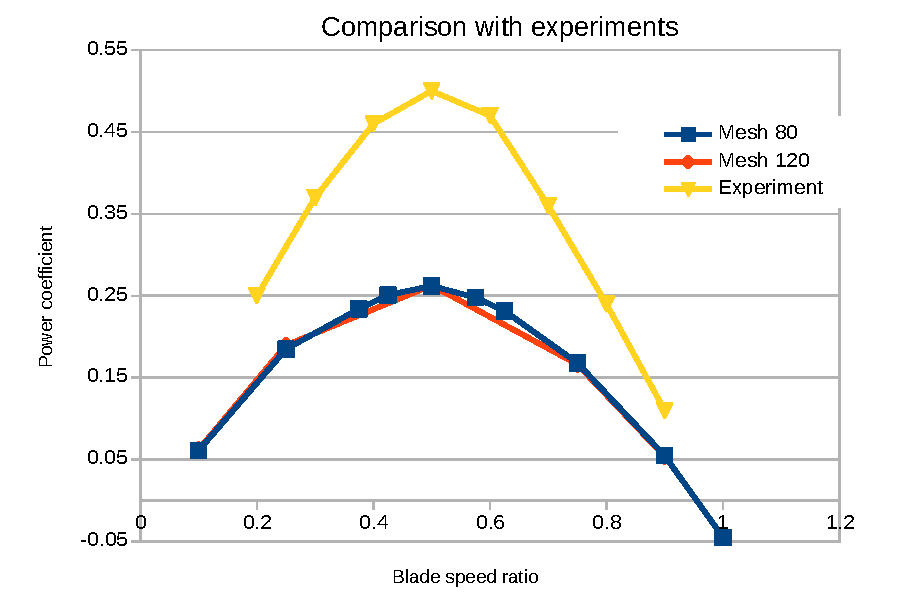
\includegraphics[width=5cm]{images/bsr/bsr-exp.pdf}
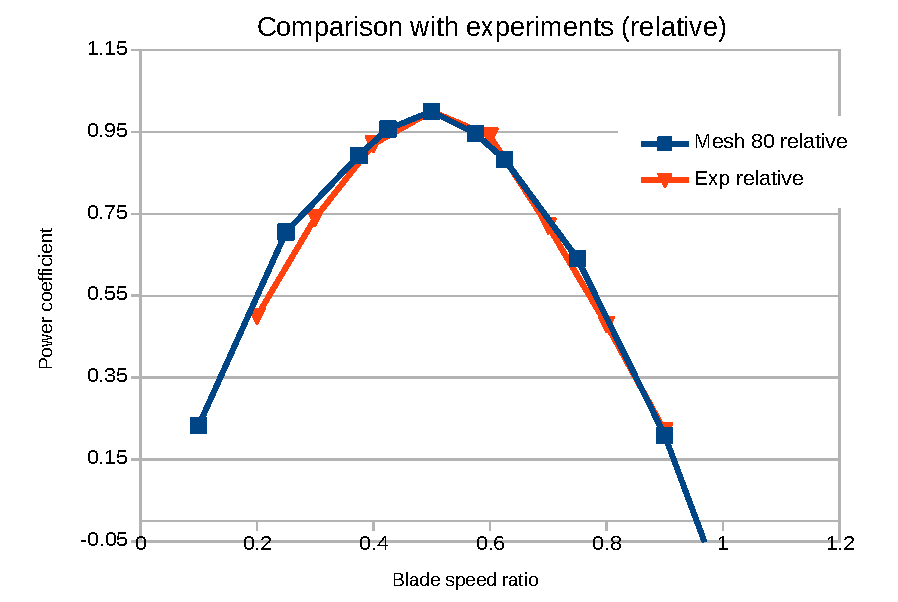
\includegraphics[width=5cm]{images/bsr/bsr-exp-relative.pdf}
%\caption{Relative comparison between mesh 80 and experimental results}
%\label{fig:bsr-comparison-exp-relative}
\end{figure}


\end{frame}

\section{Final results}


%%%%%%%%%%%%%%%%%%%%%%%%%%%%%%%%%%%%%%%%%%%%%%
\begin{frame}
\frametitle{Final results}
After the boundary enhanced analysis we have noticed that pressure residuals are not a preblem anymore.

We decided to reduce courant number to 5 since we can manage a single simulation which takes longer time.

To be sure to reach regime condition we have also increased simulation time from $2.4\s$ to $3.6\s$.

The domain has been expanded just upstream.


\begin{figure}[H]
\centering

\includegraphics[width=\textwidth]{images/final/mesh120.png}
\caption{Final mesh representation.}
\label{fig:final-mesh}
\end{figure}


\end{frame}



%%%%%%%%%%%%%%%%%%%%%%%%%%%%%%%%%%%%%%%%%%%%%%
\begin{frame}
\frametitle{Final results}

\begin{figure}[H]
\centering
\includegraphics[width=\textwidth]{images/final/{U2.4}.png}
\includegraphics[width=\textwidth]{images/final/{p2.4}.png}
\includegraphics[width=\textwidth]{images/final/{pnog2.4}.png}
%\caption{Relative comparison between mesh 80 and experimental results}
%\label{fig:final-pnog24}
\end{figure}


\end{frame}


%%%%%%%%%%%%%%%%%%%%%%%%%%%%%%%%%%%%%%%%%%%%%%
\begin{frame}
\frametitle{Final results}

For the final value of the power of this report we have decided to take the last turn that we have simulated.
\begin{center}
\textbf{Power} = $\round{4.49272061057} \w$ (Computational time $\approx$ 12h)
\end{center}

\begin{figure}[H]
\centering
\includegraphics[width=9cm]{images/final/{residuals}.png}
%\caption{Residuals of the final simulation.}
%\label{fig:final-pnog24}
\end{figure}

\end{frame}
























\end{document} 
